\chapter{Fabrication} \label{Fabrication}

Metal fabrication is the creation of metal structures by cutting, welding, bending, machining and assembling processes. It is a value added process involving the creation of machines, parts, and structures from various raw materials. As with other manufacturing processes, both human labour and automation are commonly used.

Machining is a specialized trade of removing material from a block of metal to make it a desired shape, using metal lathes, mills, drills, and other portable machining tools. Most solid components, such as gears, bolts, screws and nuts, are machined. Welding is the main focus of steel fabrication. Formed and machined parts are later assembled and tack-welded in place, then rechecked for accuracy.


\section{Components to be Assembled} \label{Components to be Assembled}

% Please add the following required packages to your document preamble:
% \usepackage{graphicx}
\begin{table}[!ht]
\centering
%\resizebox{\textwidth}{!}{%
\begin{tabular}{|l|l|l|c|} 
\hline
\begin{tabular}[c]{@{}l@{}}Sr.\\ No.\end{tabular} & Component                & \begin{tabular}[c]{@{}l@{}}Dimensions\\ (mm)\end{tabular} & \multicolumn{1}{l|}{Quantity}  \\ 
\hline
1                                                 & Main Frame               & 945*565*800                                               & 1                              \\ 
\hline
2                                                 & Bottom Plate             & 600*580*1                                                 & 1                              \\ 
\hline
3                                                 & Front Scraper            & 40*40*1                                                   & 1                              \\ 
\hline
4                                                 & Blade                    & 460*10*70                                                 & 12                             \\ 
\hline
5                                                 & Main Shaft               & Ø30                                                       & 1                              \\ 
\hline
6                                                 & Roller Shaft             & Ø25                                                       & 2                              \\ 
\hline
\multirow{}{}{7}                                & \multirow{}{}{Chains}  & 2200                                                      & 2                              \\ 
\cline{3-4}
                                                  &                          & 500                                                       & 1                              \\ 
\hline
8                                                 & Sprocket                 & 9 teeth                                                   & 4                              \\ 
\hline
9                                                 & Free Wheel               & 18 teeth                                                  & 2                              \\ 
\hline
\multirow{}{}{10}                               & \multirow{}{}{Bearing} & Ø30*Ø55*13                                                & 2                              \\ 
\cline{3-4}
                                                  &                          & Ø25*Ø47*12                                                & 4                              \\ 
\hline
11                                                & Omnidirectional Wheels   & \multicolumn{1}{c|}{Ø155*30}                              & 2                              \\ 
\hline
12                                                & Rubber Wheels            & \multicolumn{1}{c|}{Ø155*25}                              & 2                              \\
\hline
\end{tabular}
%
%}
\caption{Components to be Assembled}
\label{tab:Components to be Assembled}
\end{table}













\section{Manufacturing Operations Used} \label{Manufacturing Operations Used}
\subsection{Cutting} \label{Cutting}
Cutting process encompasses a wide variety of equipment used to remove metal from the work piece. Any basic cutting operation involves a cutting tool that is mostly a disc made out of abrasive material.The cutting equipment used in fabrication of this project are chop saw and angle grinder.

\subsubsection{Chop Saw} \label{Chop Saw}
This is a power tool that is used on larger work-pieces. It has a hinge like arm on which the blade is mounted. It can be used on variety of materials provided the right cutting blade is used. Chop saws can be used to cut materials as soft as wood and as hard as structural grade steel. It has a provision on the bed where the job is placed and holds the piece tightly. It also allows to set angles to take angled cuts. The chop saw is used mainly to take perfectly straight cuts on metal tubes or bar stocks.

Chop saw was used to cut the rectangular stainless steel rods into required sizes and angles for fabricating the main frame.It was also used to cut the cylindrical stainless steel rods according to the required dimensions to use them as shafts. 

\begin{figure}[h!]
    \centering
    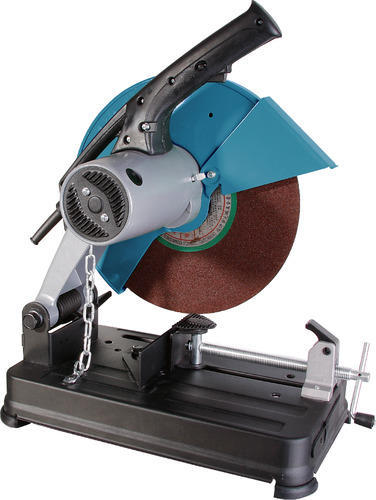
\includegraphics{chopsaw.jpg}
    \caption{Chop Saw}
    \label{fig:Chop Saw}
\end{figure}

\subsubsection{Angle Grinder} \label{Angle Grinder}
This is a versatile machining tool that allows a number of attachments that can be used for various operations. The angle grinder can be fitted with a grinding disc for grinding purposes, cutting disc for cutting, a wire brush attachment used to scrub of surface level rust and various other attachments. Cutting blades comes in a variety of options depending on the metal that has to be cut.

By attaching a suitable cutting disc attachment the angle grinder was used to cut the stainless steel sheets and CRCA steel sheets according to our required dimensions to utilize them for making the bottom plate, front scraper, blades and the side panels.

\begin{figure}[h!]
    \centering
    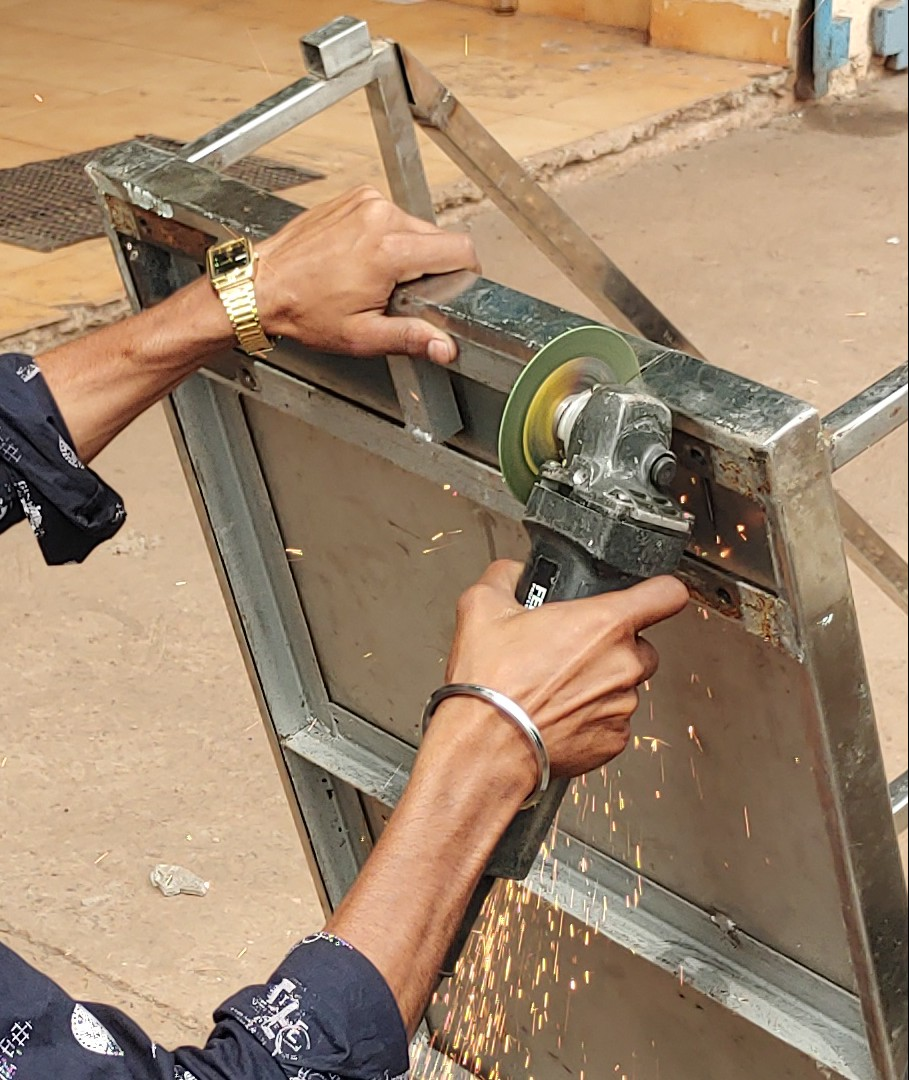
\includegraphics[scale=0.1]{cutting.jpg}
    \caption{Angle Grinder}
    \label{fig:Angle Grinder}
\end{figure}





\subsection{Welding} \label{Welding}
Welding is a fabrication process that joins materials,usually metals or thermoplastics, by using high heat to melt the parts together and allowing them to cool, causing fusion.Arc welding was used during fabrication of this project.

\subsubsection{Arc Welding} \label{Arc Welding}
Arc welding is a type of welding that uses a welding power supply to create an electric arc between an electrode and the base material to melt the metals at the welding point. They can use either direct (DC) or alternating (AC) current, and consumable or non consumable electrodes. The welding region is usually protected by some type of shielding gas, vapour or slag. Arc welding processes may be manual, semi automatic, or fully automated.

An electric current is used to strike an arc between the base material and a consumable electrode rod or stick. The electrode rod is made of a material that is compatible with the base material being welded and is covered with a flux that gives off vapours that serve as a shielding gas and provide a layer of slag, both of which protect the weld area from atmospheric contamination. The electrode pour itself acts as a filler material, making separate filler unnecessary. The process is very versatile, requiring little operator training and inexpensive equipment. However, weld times are rather slow, since the consumable electrodes must be frequently replaced and because slag, the residue from the flux, must be chipped away after welding.

The main frame was build by joining the stainless steel rods together by welding. The bottom plate, scraper and the the mounts to hold the shafts were permanently attached to the main frame by welding. Also the blades were welded to the chains to form the scraping mechanism.  

\begin{figure}[H]
    \centering
    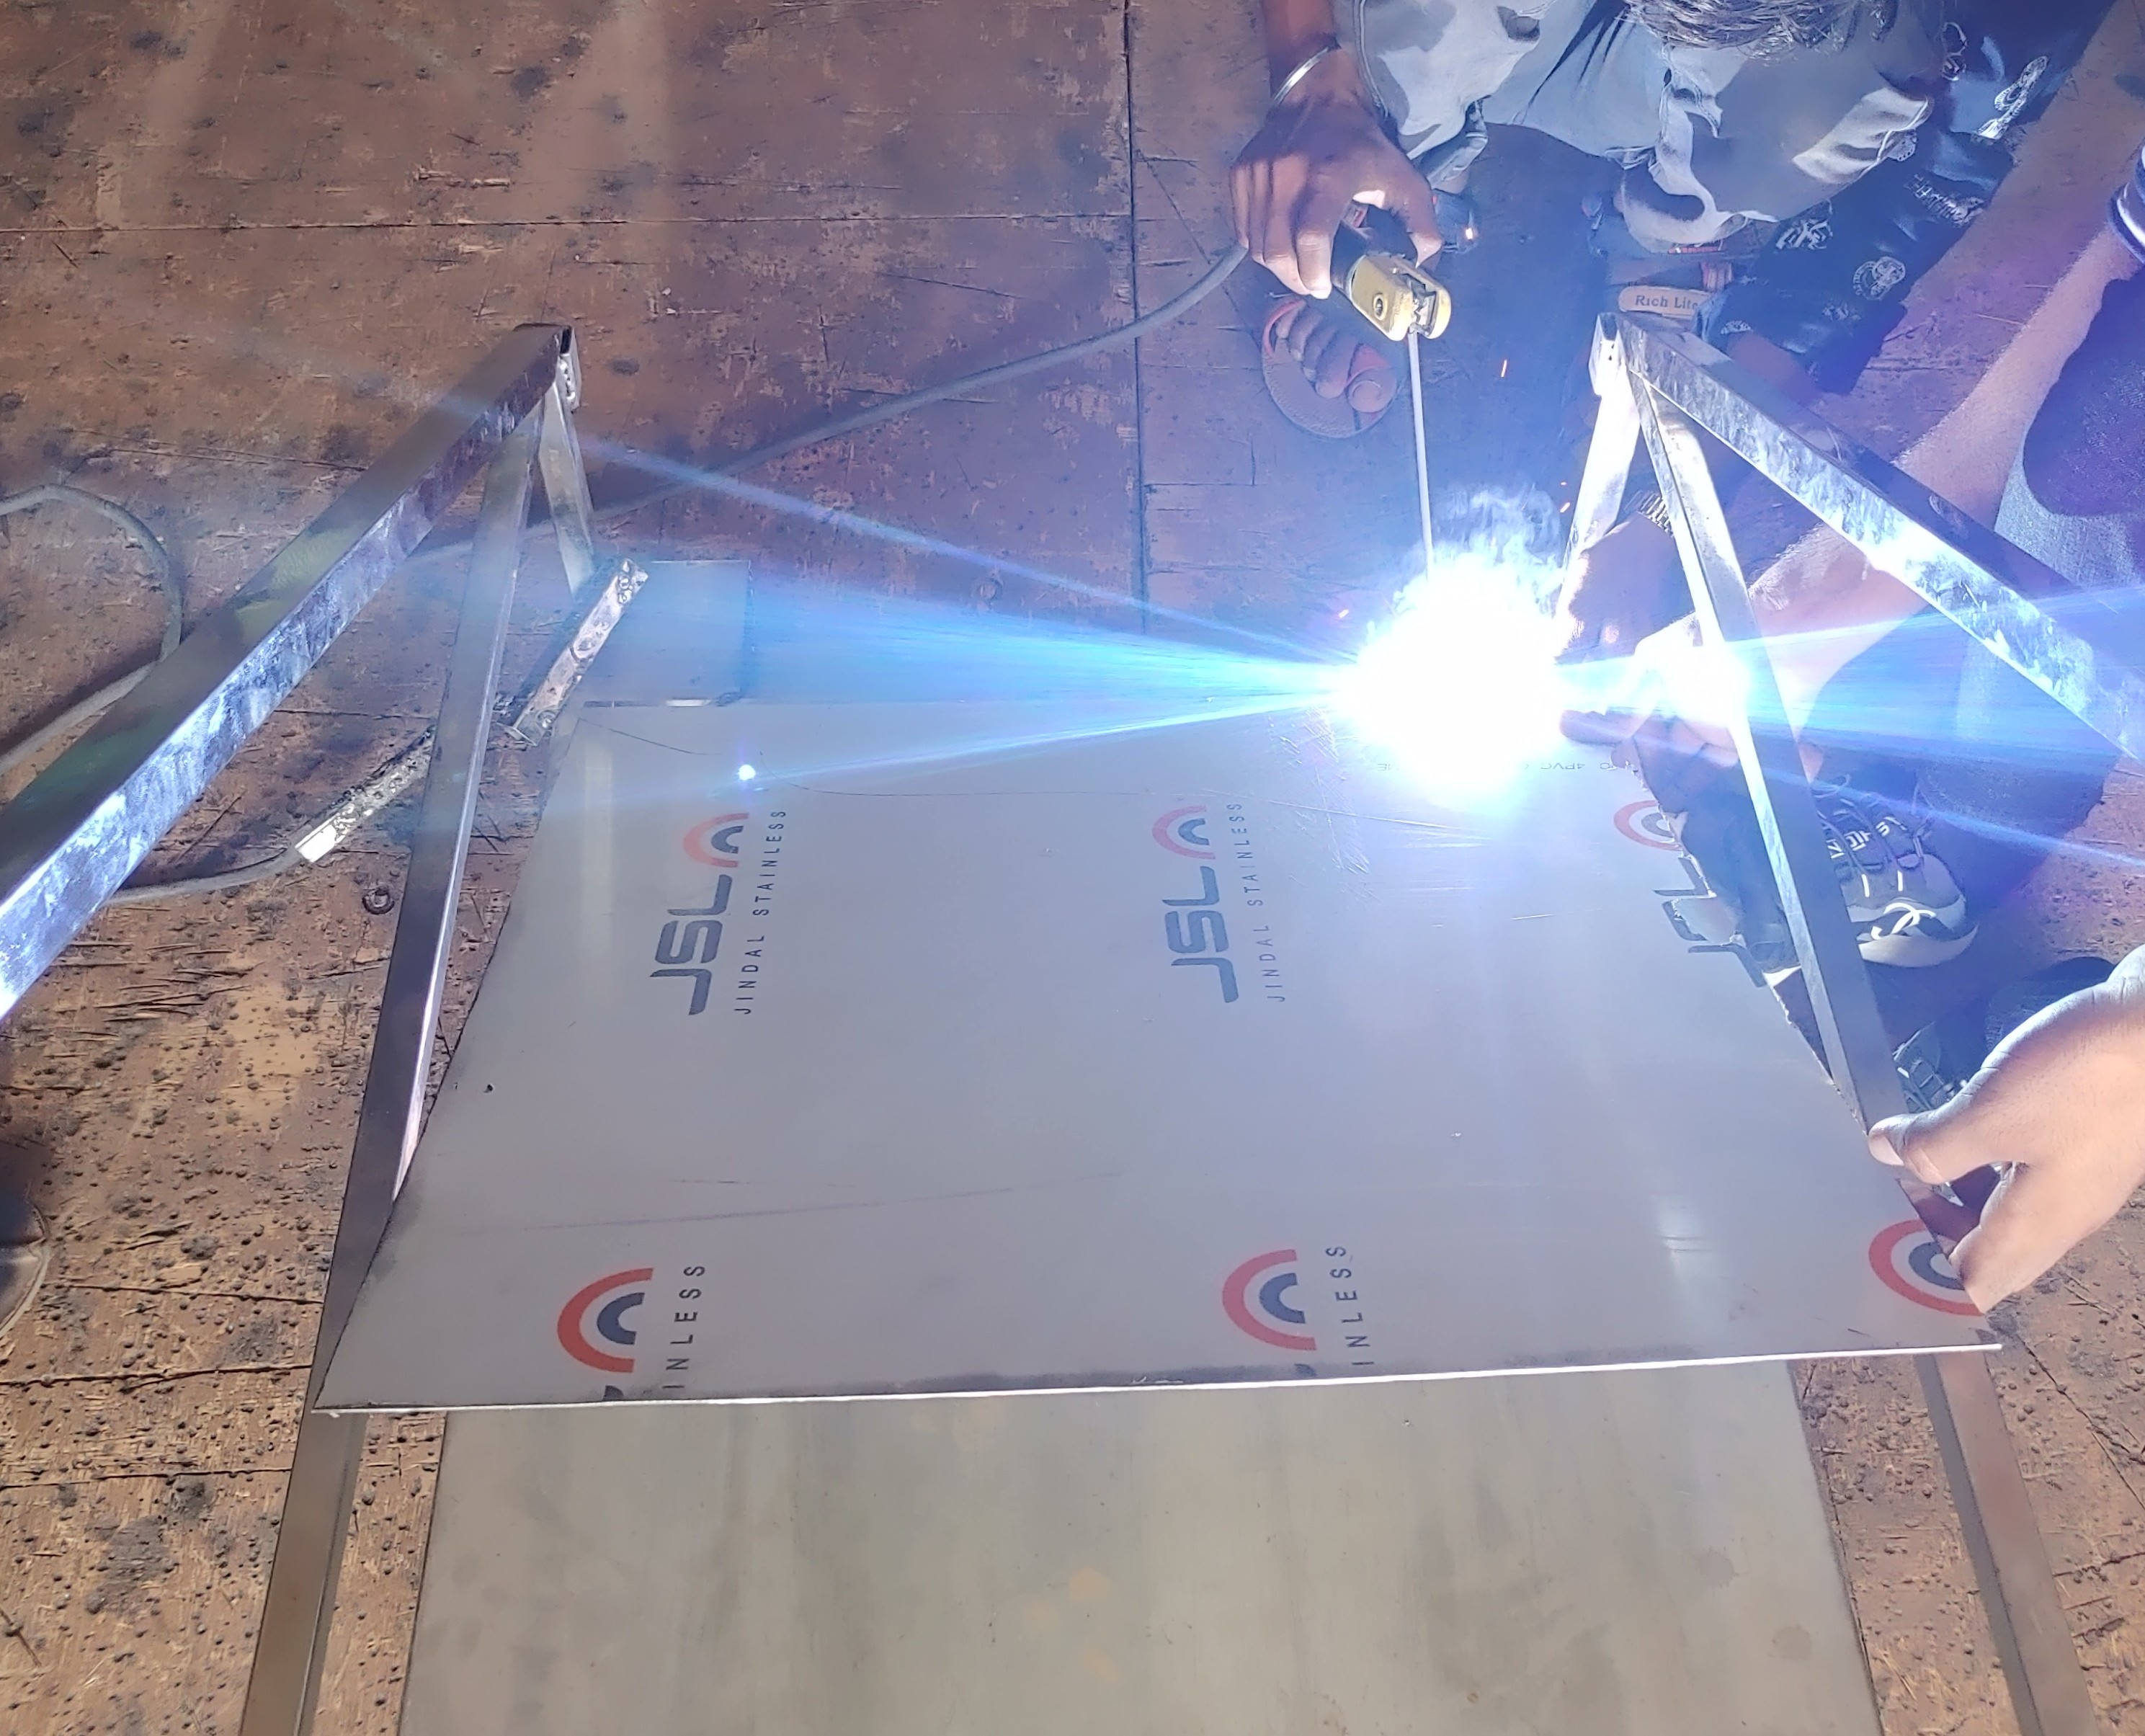
\includegraphics[scale=0.05]{welding.jpg}
    \caption{Welding}
    \label{fig:Welding}
\end{figure}

\subsection{Grinding} \label{Grinding}
Grinding is a machining process that uses abrasive material to remove surface level material from the work piece. It is actually a cutting process as this process in reality cuts the metal. On a microscopic level, grinding operation makes cuts on grain level similar to how cutting operation would cut a small chip off of a metal. It can be used for jobs that demand fine and accurate machining along with large input of manpower and it also can be applied to work just as good in a mass production system to machine large volumes of material off or do a fine job.

It is now relatively simple to work with hard materials thanks to recent advancements in machining techniques and new age processes. However, prior to these developments, grinding was the only machining process capable of handling materials as hard as hardened steel. The grinding machines used in fabrication of this project are angle grinder and pedestal grinder.

\subsubsection{Angle Grinder} 

The angle grinder is a handheld device that can be used for both cutting and grinding. The motor in the device spins in an axis running along the length of the device. A gearing setup is used to change the axis of motor drive axis and turn it by 90 degrees. The disc blades for grinding or for cutting are mounted on a shaft. Angle grinders are provided with a guard that prevents the operator to touch the blade. It also shields the operator from the sparks that are caused during machining.

By attaching a suitable grinding disc attachment the angle grinder was used to remove the slag left after welding to provide smooth surface finish.

\subsubsection{Pedestal Grinder}
These are extremely rugged and robust in design. They are used for heavy duty machining The main body of the machine is made from cast iron. It is firmly bolted on ground making sure that it would never move or budge while in operation. The main body houses a motor that drives the grinding disc. The grinding disc is made of abrasive material.
Pedestal grinder was required to sharpen the cutting tool so that the boring of sprockets and freewheel mounts was accurate to dimension and had a smooth surface finish.

\begin{figure}[H]
    \centering
    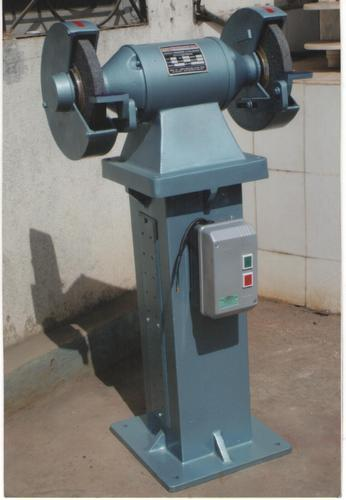
\includegraphics[scale=0.3]{Grinder.jpg}
    \caption{Pedestal Grinder}
    \label{fig:Pedestal Grinder}
\end{figure}


\subsection{Drilling} \label{Drilling}

It is a machining process used to make holes into the work piece. Drilling uses drill bits to cut the holes of circular cross section. The working of the drill is simple. A drill bit is held by the chuck. The drill chuck is mounted on a shaft that is connected to the shaft of the motor or is the shaft of the motor. The motor rotates at very high rpm causing the drill bit to rotate as well. Drill bits vary in function, shape, size, material and cutting pattern depending on the requirement of job at hand. The axis of rotation of the drill bit has to be perpendicular to the surface of the work piece for the hole to be perfectly cut. The two predominantly used drilling equipment used in industry are hand drilling and vertical drilling.Hand drilling was employed during fabrication of this project.

\subsubsection{Hand Drilling} \label{Hand Drilling}

These are the most common and widely used drilling machines. These drills have pistol grips with a trigger for turning it on. Hand drills come in a huge variety of sizes, speed and torque. A universal motor is used as it has a high power to weight ratio. Hand drills can handle a variety of attachments as well, like orbital sanders, power saws, wire brush attachment and even grinding bits made out of hard abrasive material. Depending on the size of the drill and the chuck on it, the drill bits for drilling are used. A regular hand drill can be used with a drill bit up to 12mm in diameter.

Holes were drilled on the bottom of the frame with hand drill machine to attach the omnidirectional wheels to the frame with nuts and bolts. 

\begin{figure}[h!]
    \centering
    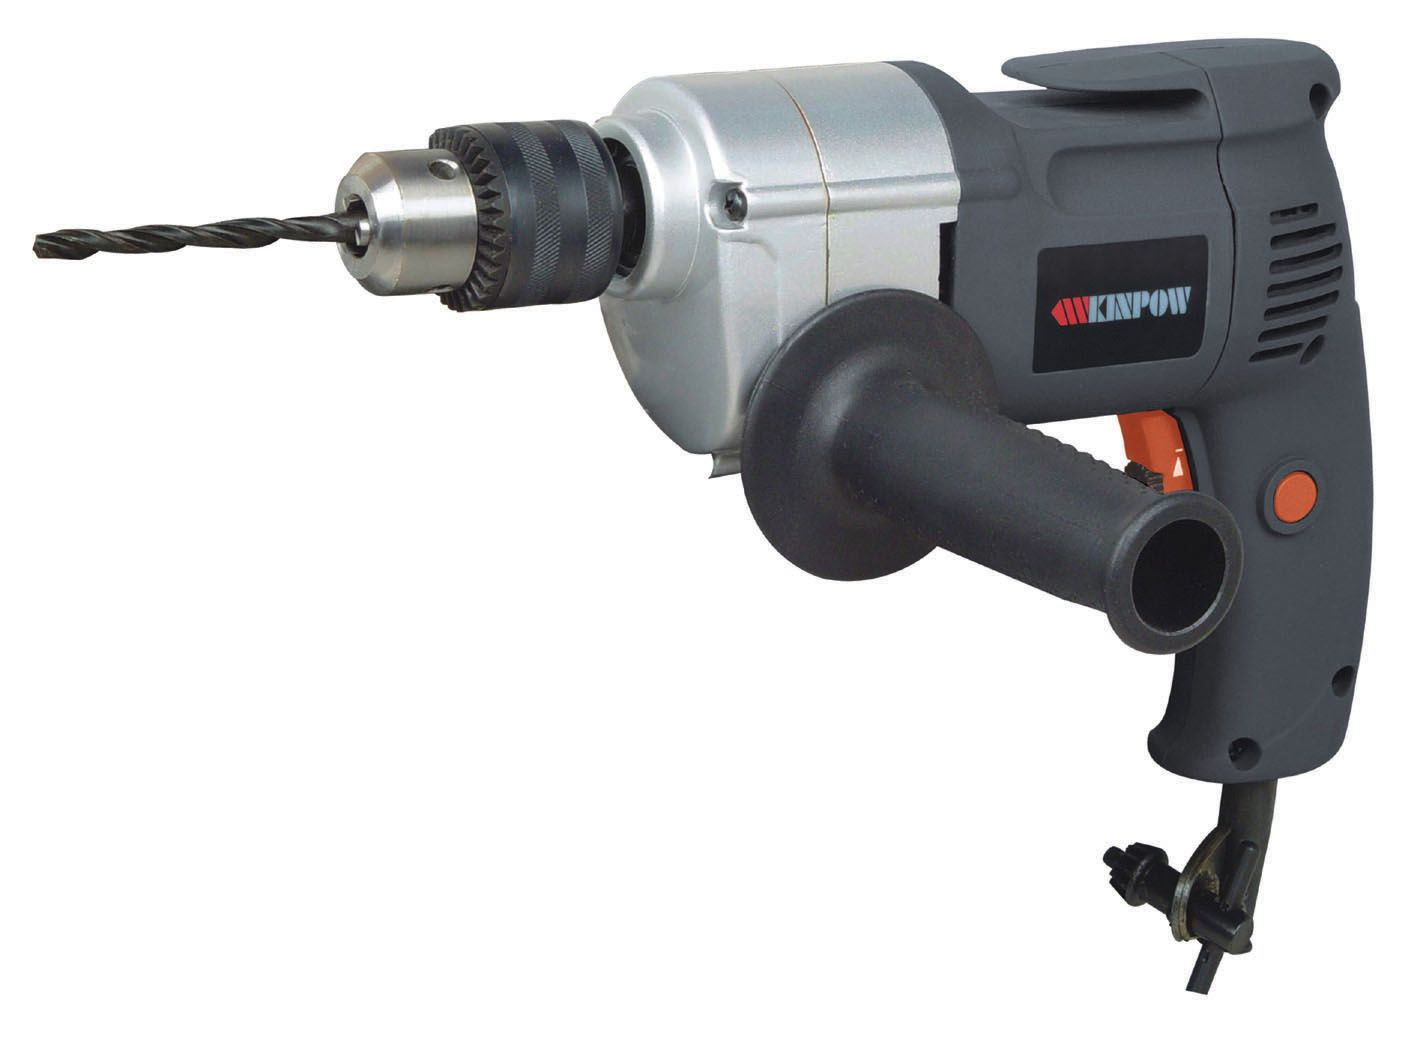
\includegraphics[scale=0.5]{Hand drill machine.jpg}
    \caption{Hand Drill Machine}
    \label{fig:Hand Drill Machine}
\end{figure}



\subsection{Turning} \label{Turning}
Turning is a machining process in which a cutting tool, typically a non rotary tool bit, describes a helical tool path by moving more or less linearly while the work-piece rotates. The tool's axes of movement may be a straight line, or they may be along some set of curves or angles, but they are essentially linear. Usually the term turning is reserved for the generation of external surfaces by the cutting action, whereas this same essential cutting action when applied to internal surfaces is called "boring". The cutting of faces on the work piece (i.e. surfaces perpendicular to its rotating axis), whether with a turning or boring tool, is called "facing".

Turning can be done manually, in a traditional form by lathe, which frequently requires continuous supervision by the operator, or by using an automated lathe which does not. Today the most common type of such automation is computer numerical control, better known as CNC.

When turning, a piece of relatively rigid material (such as wood, metal, plastic or stone) is rotated and a cutting tool is traversed along 1, 2 or 3 axis of motion to produce precise diameters and depths. Turning can be either on the outside of the cylinder or on the inside (also known as boring) to produce tubular components to various geometries.

The turning processes are typically carried out on lathe, considered to be the oldest machine tools, and can be of four different types such as straight turning, taper turning, profiling or external grooving. Those types of turning processes can produce various shapes of materials such as straight, conical, curved or grooved work piece. In general, turning uses single point cutting tools.

\subsection{Boring} \label{Boring}
In machining, boring is the process of enlarging a hole that has already been drilled (or cast), by means of a single-point cutting tool. Boring is used to achieve greater accuracy of the diameter of a hole, and can be used to cut a tapered hole. Boring can be viewed as the internal-diameter counterpart to turning, which cuts external diameters.

There are various types of boring. The boring bar may be supported on both ends (which only works if the existing hole is a through hole), or it may be supported at one end (which works for both through holes and blind holes) Line boring implies the former. Back boring is the process of reaching through an existing hole and then boring on the "back" side of the work-piece (relative to the machine headstock).

The boring process can be executed on various machine tools including general purpose or universal machines, such as lathes (turning centres) or milling machine(machining centres). and machines designed to specialize in boring as a primary function, such as jig borers and boring machines or boring mills, which include vertical boring mills (work-piece rotates around a vertical axis while boring bar/head moves linearly; essentially a vertical lathe) and horizontal boring mills (work-piece sits on a table while the boring bar rotates around a horizontal axis; essentially a specialized horizontal milling machine).

The boring process was used to make a hole on the rubber tyres so that it can be mounted on the shaft.This tyres are used as the front tyres for the cow dung collecting system.

\begin{figure}[h!]
    \centering
    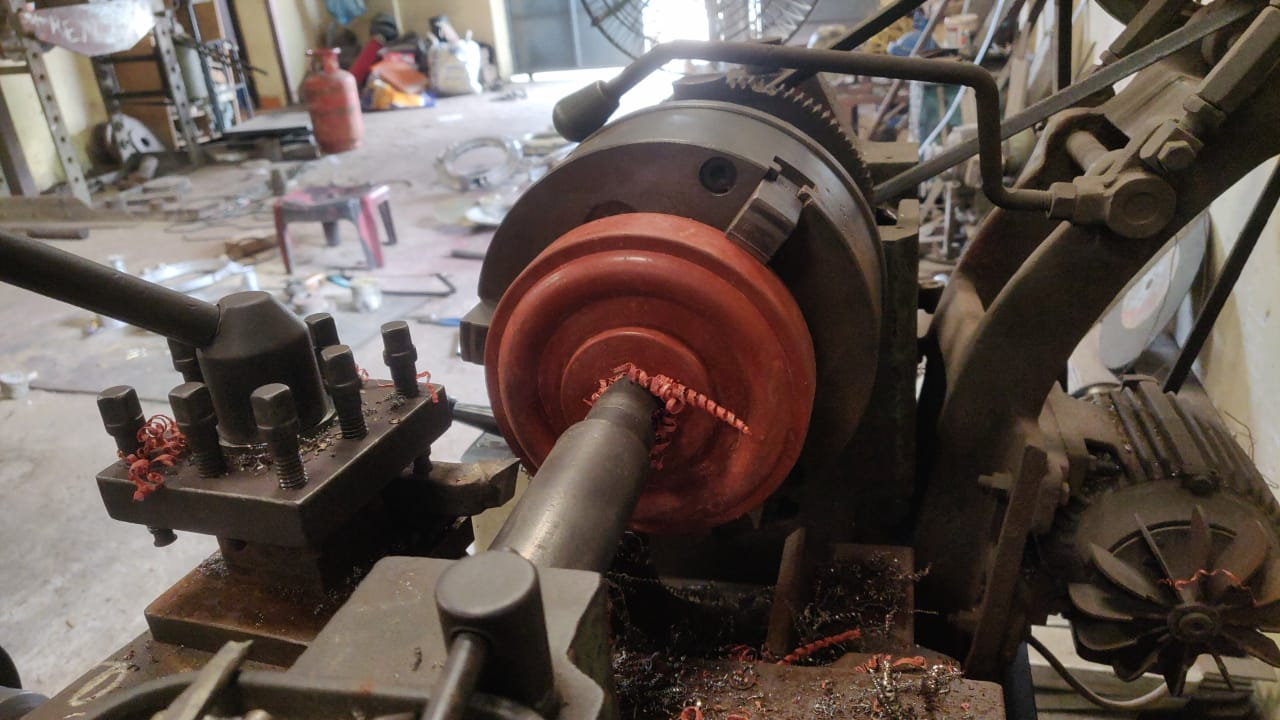
\includegraphics[scale=0.15]{Boring.jpg}
    \caption{Boring}
    \label{fig:Boring}
\end{figure}

\section{Fabrication Process} \label{Fabrication Process}

A base plate was developed by taking a SS sheet and welding support rods to it (Fig. \ref{fig:Base Plate}). This acts as the foundation for the frame.It holds the load of the collected cow dung.

The main frame (Fig. \ref{fig:Main Frame}) was build by welding the SS rods on top of the base plate  as per the CAD designs.

\begin{figure}[H]
  \centering
    \begin{minipage}{0.55\textwidth}
    \centering
      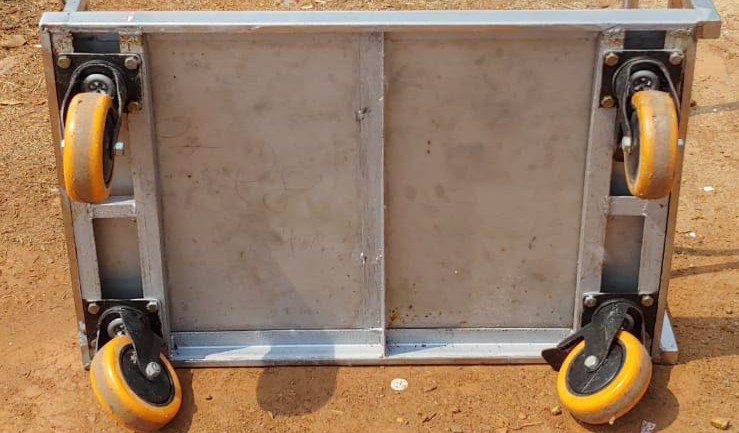
\includegraphics[width=1\textwidth]{Base plate.jpg}
      \caption{Base Plate}
      \label{fig:Base Plate}
    \end{minipage}
\hfill
    \begin{minipage}{0.30\textwidth}
    \centering
      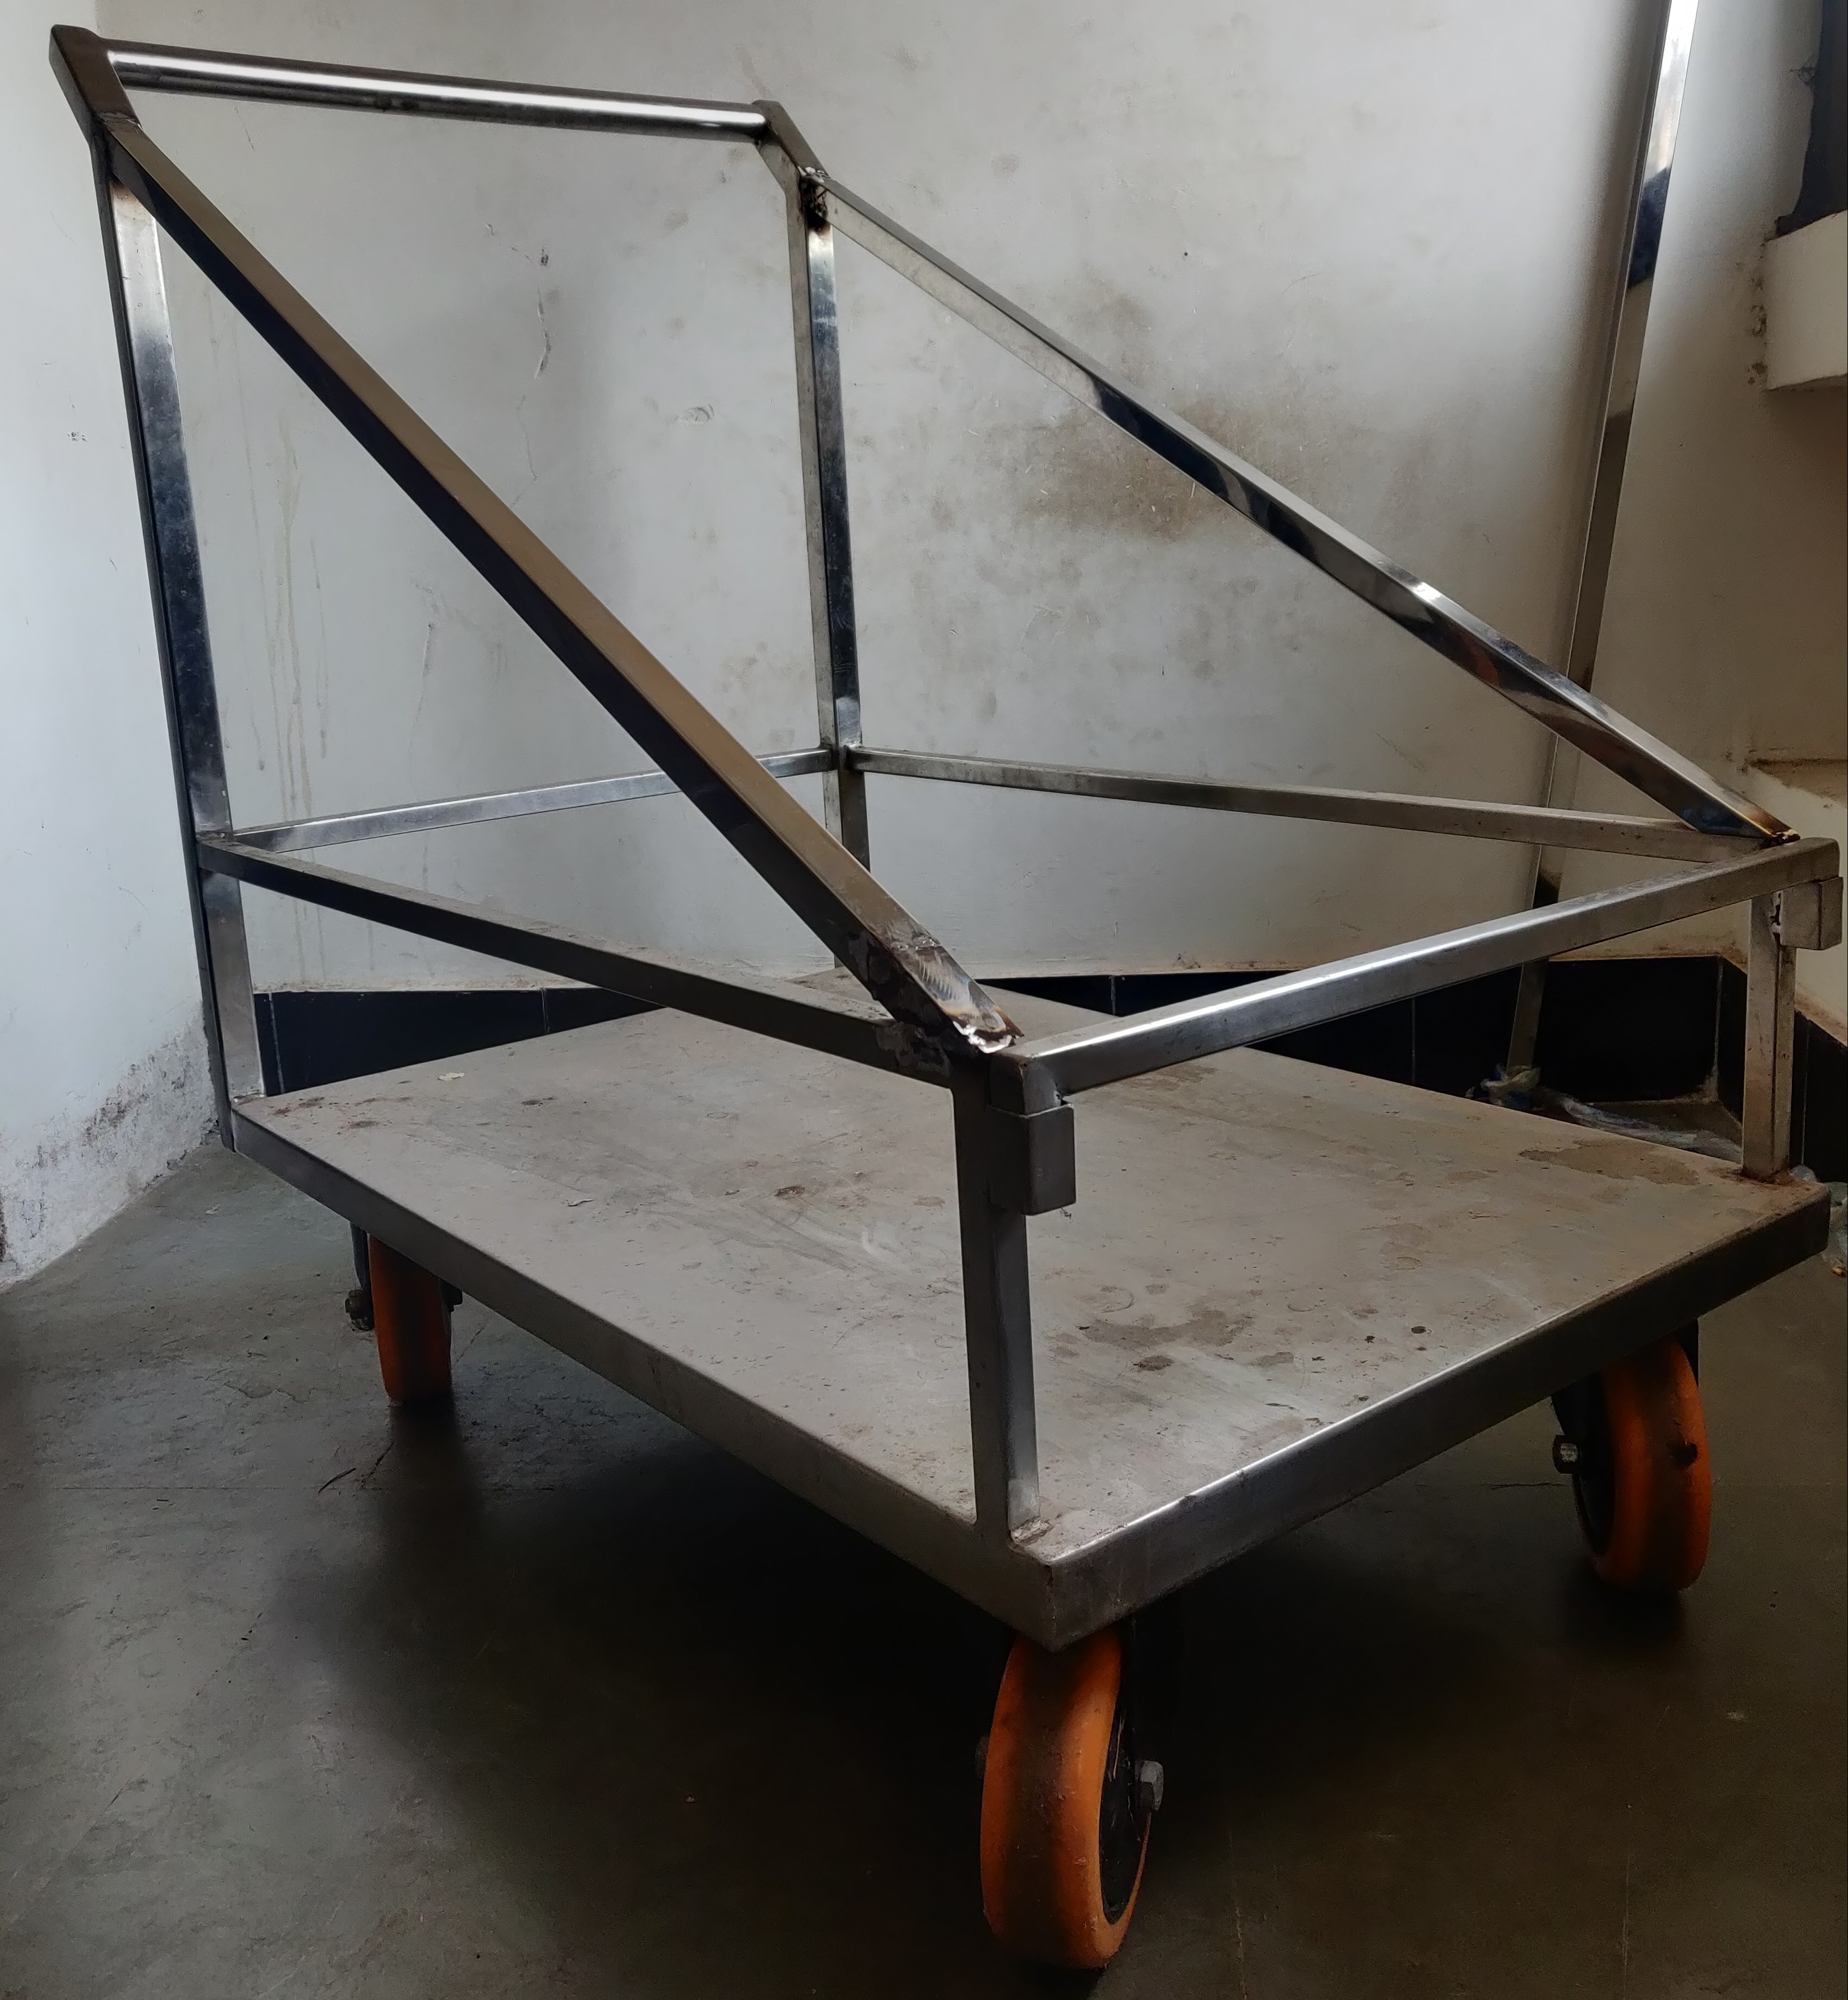
\includegraphics[width=1\textwidth]{Main Frame.jpg}
      \caption{Main Frame}
      \label{fig:Main Frame}
    \end{minipage}
\end{figure}

A bottom plate, front scraper and  four circular mounts to hold the roller shafts were welded to the main frame (Fig. \ref{fig:Assembly}). Two U mounts were welded to the bottom of the main frame to hold the main shaft (Fig. \ref{fig:U Mount}).


\begin{figure}[H]
  \centering
    \begin{minipage}{0.40\textwidth}
    \centering
      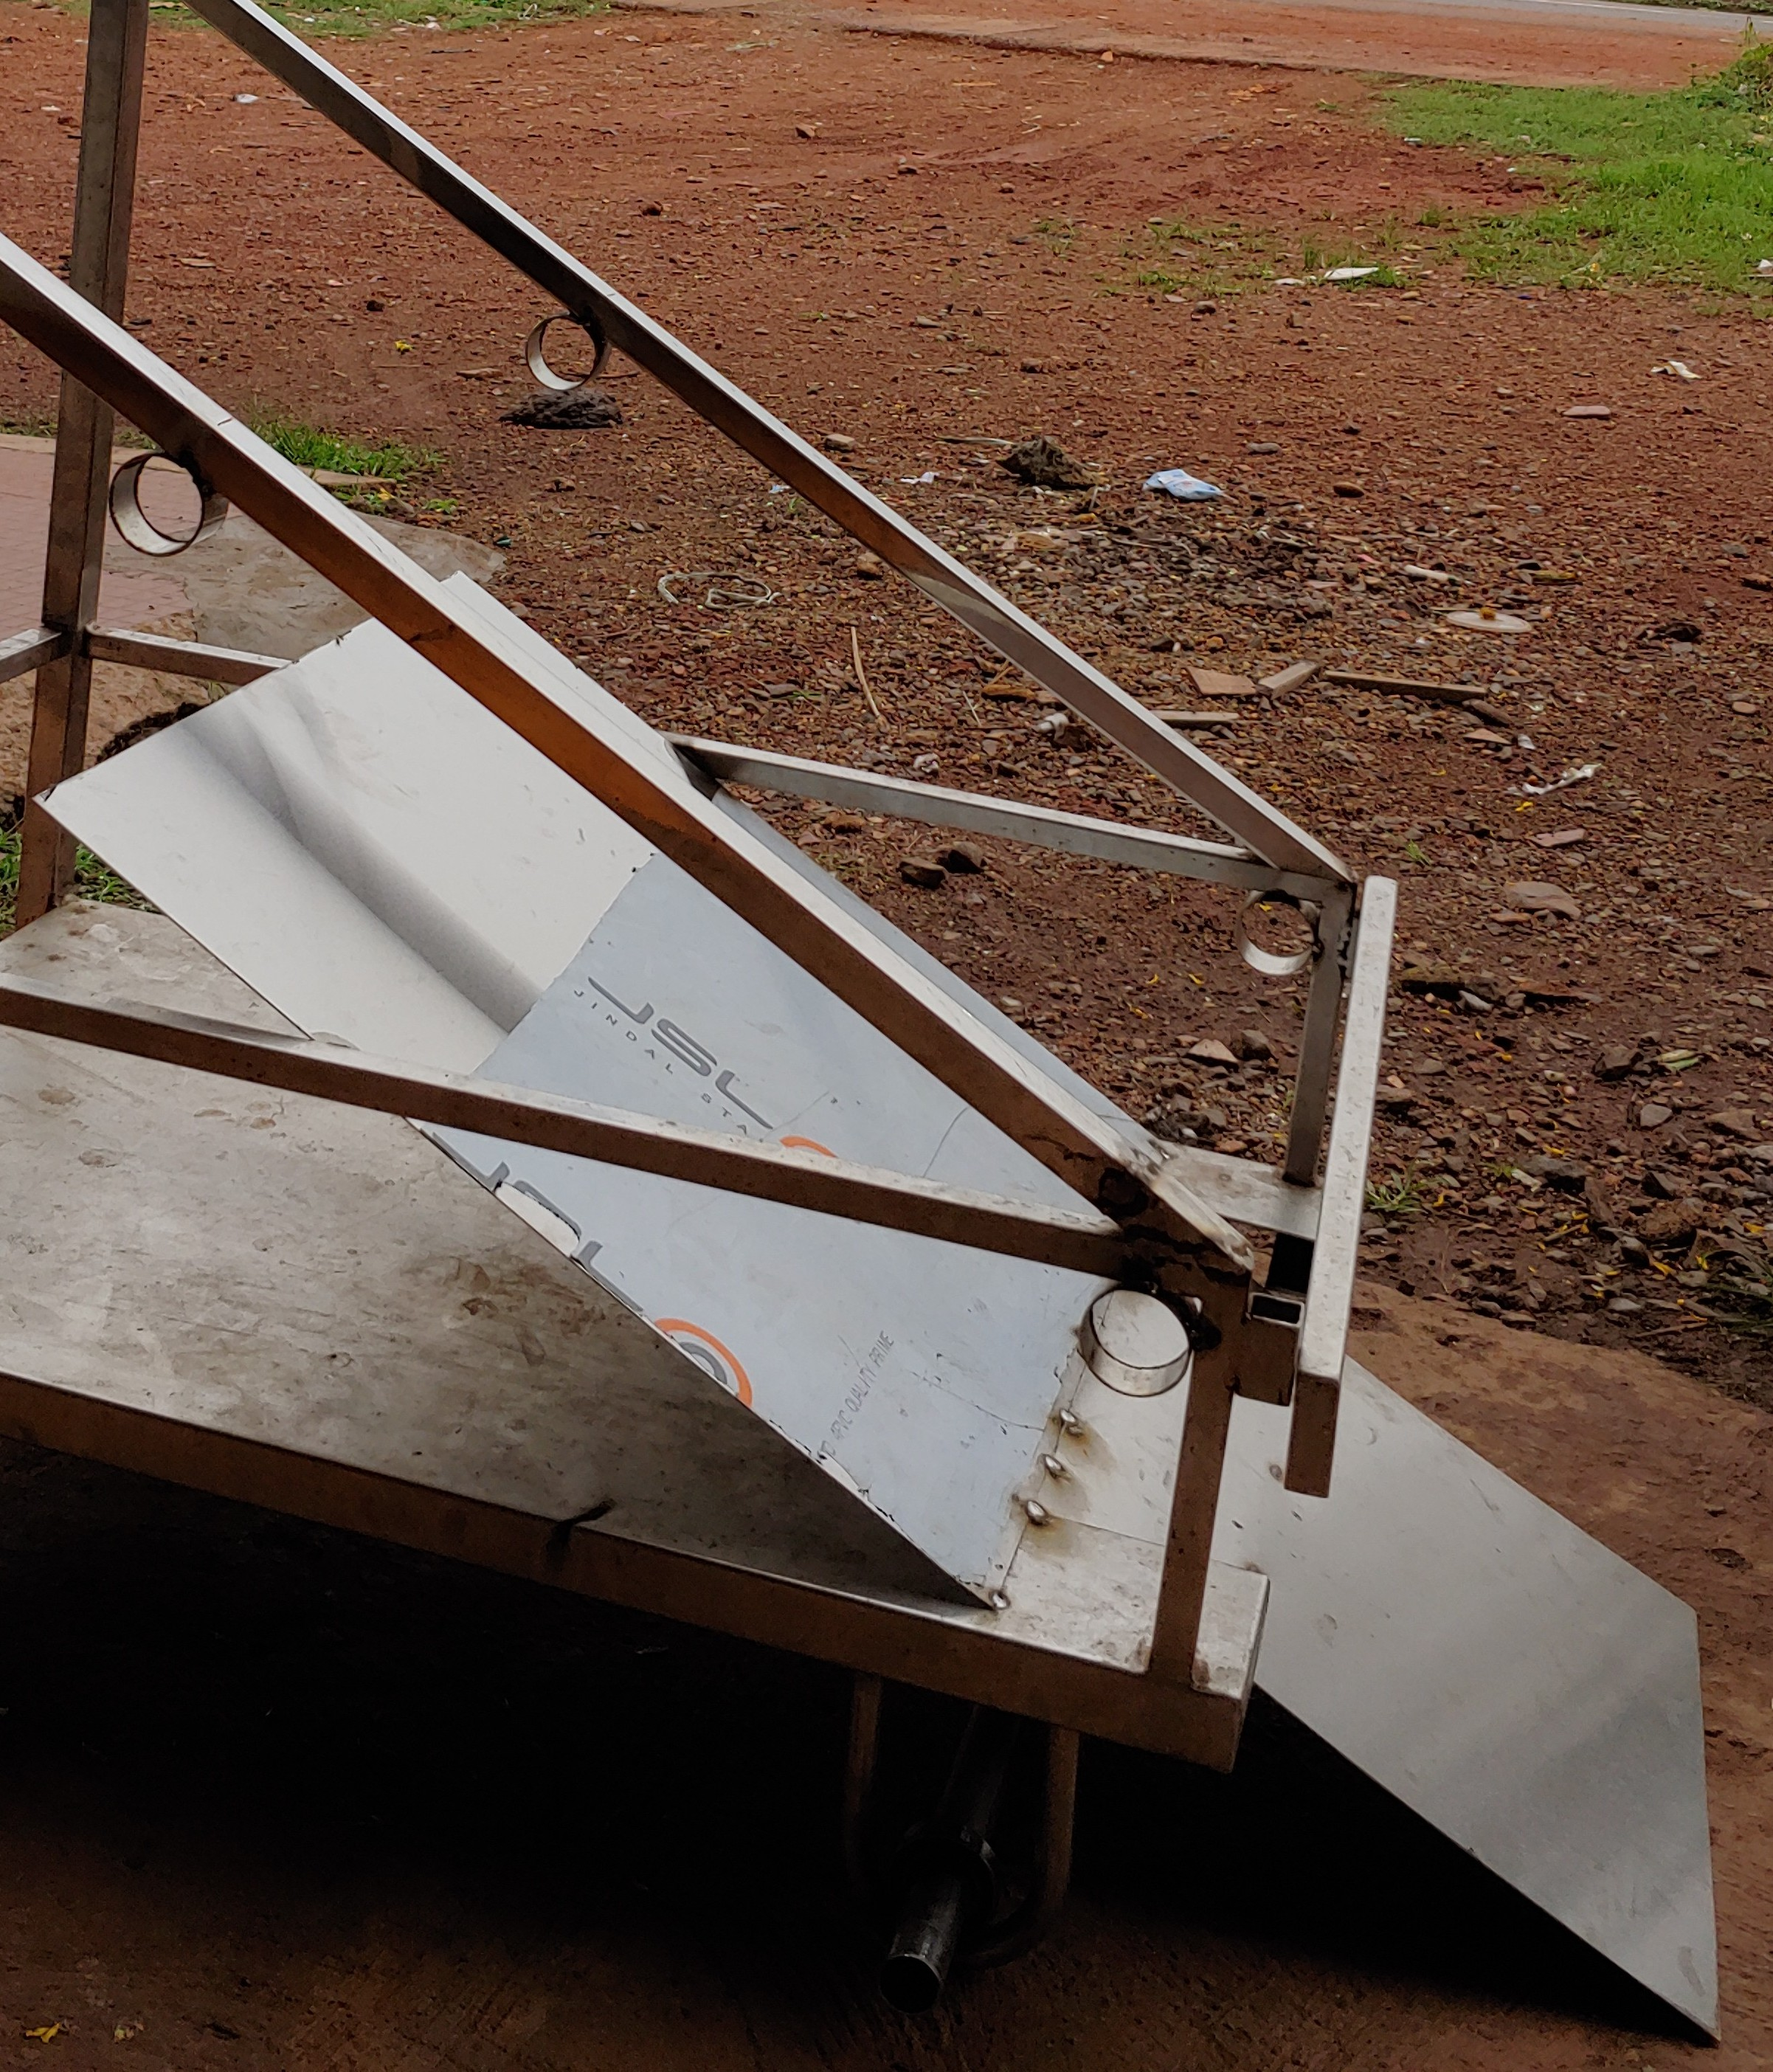
\includegraphics[width=1\textwidth]{med ass.jpg}
       \caption{Assembly}
    \label{fig:Assembly}
    \end{minipage}
\hfill
    \begin{minipage}{0.37\textwidth}
    \centering
      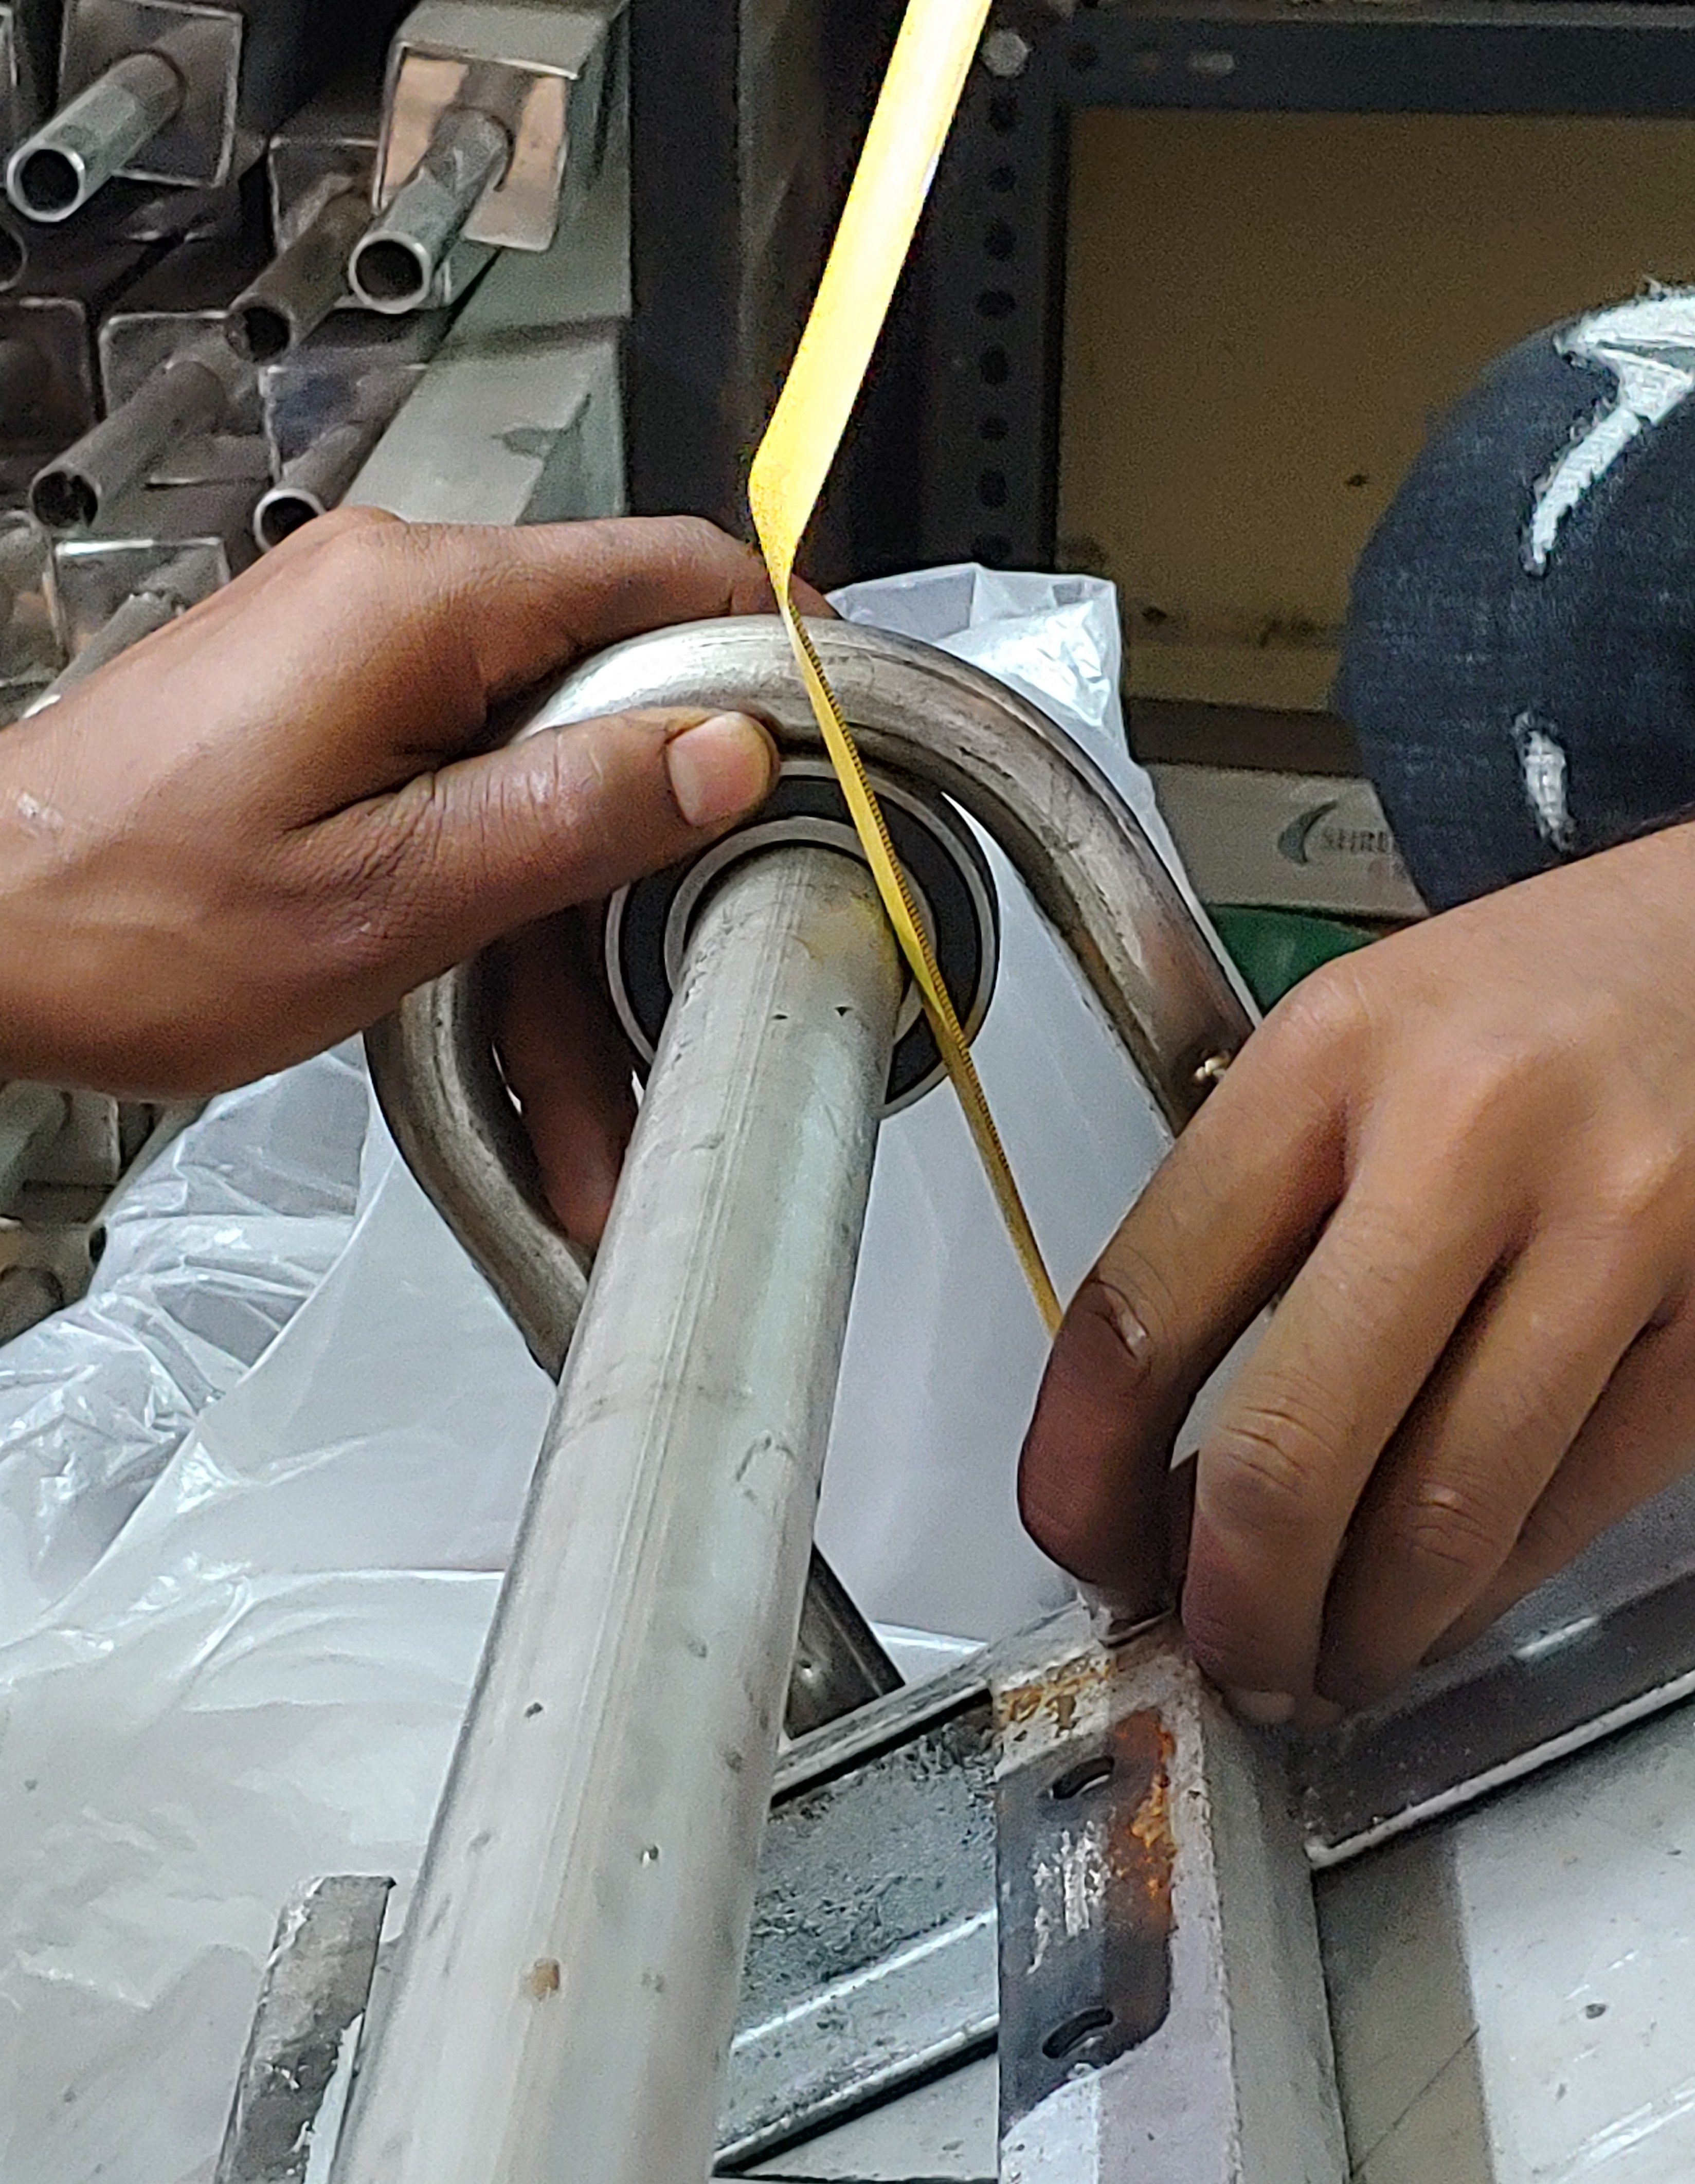
\includegraphics[width=1\textwidth]{U Mount.jpg}
      \caption{U Mount}
      \label{fig:U Mount}
    \end{minipage}
\end{figure}


Bearings were mounted on the main shaft (Fig. \ref{fig:Bearings on main shaft}) and this assembly was welded to the U mounts with weld contact between the bearing and the U mount (Fig. \ref{fig:Mounts}). Rubber tyres were mounted on the main shaft by achieving perfect interference fit between the bored diameter of the tyre and the external diameter of the main shaft (Fig. \ref{fig:Tyres assembly}).

\begin{figure}[H]
  \centering
    \begin{minipage}{0.23\textwidth}
    \centering
      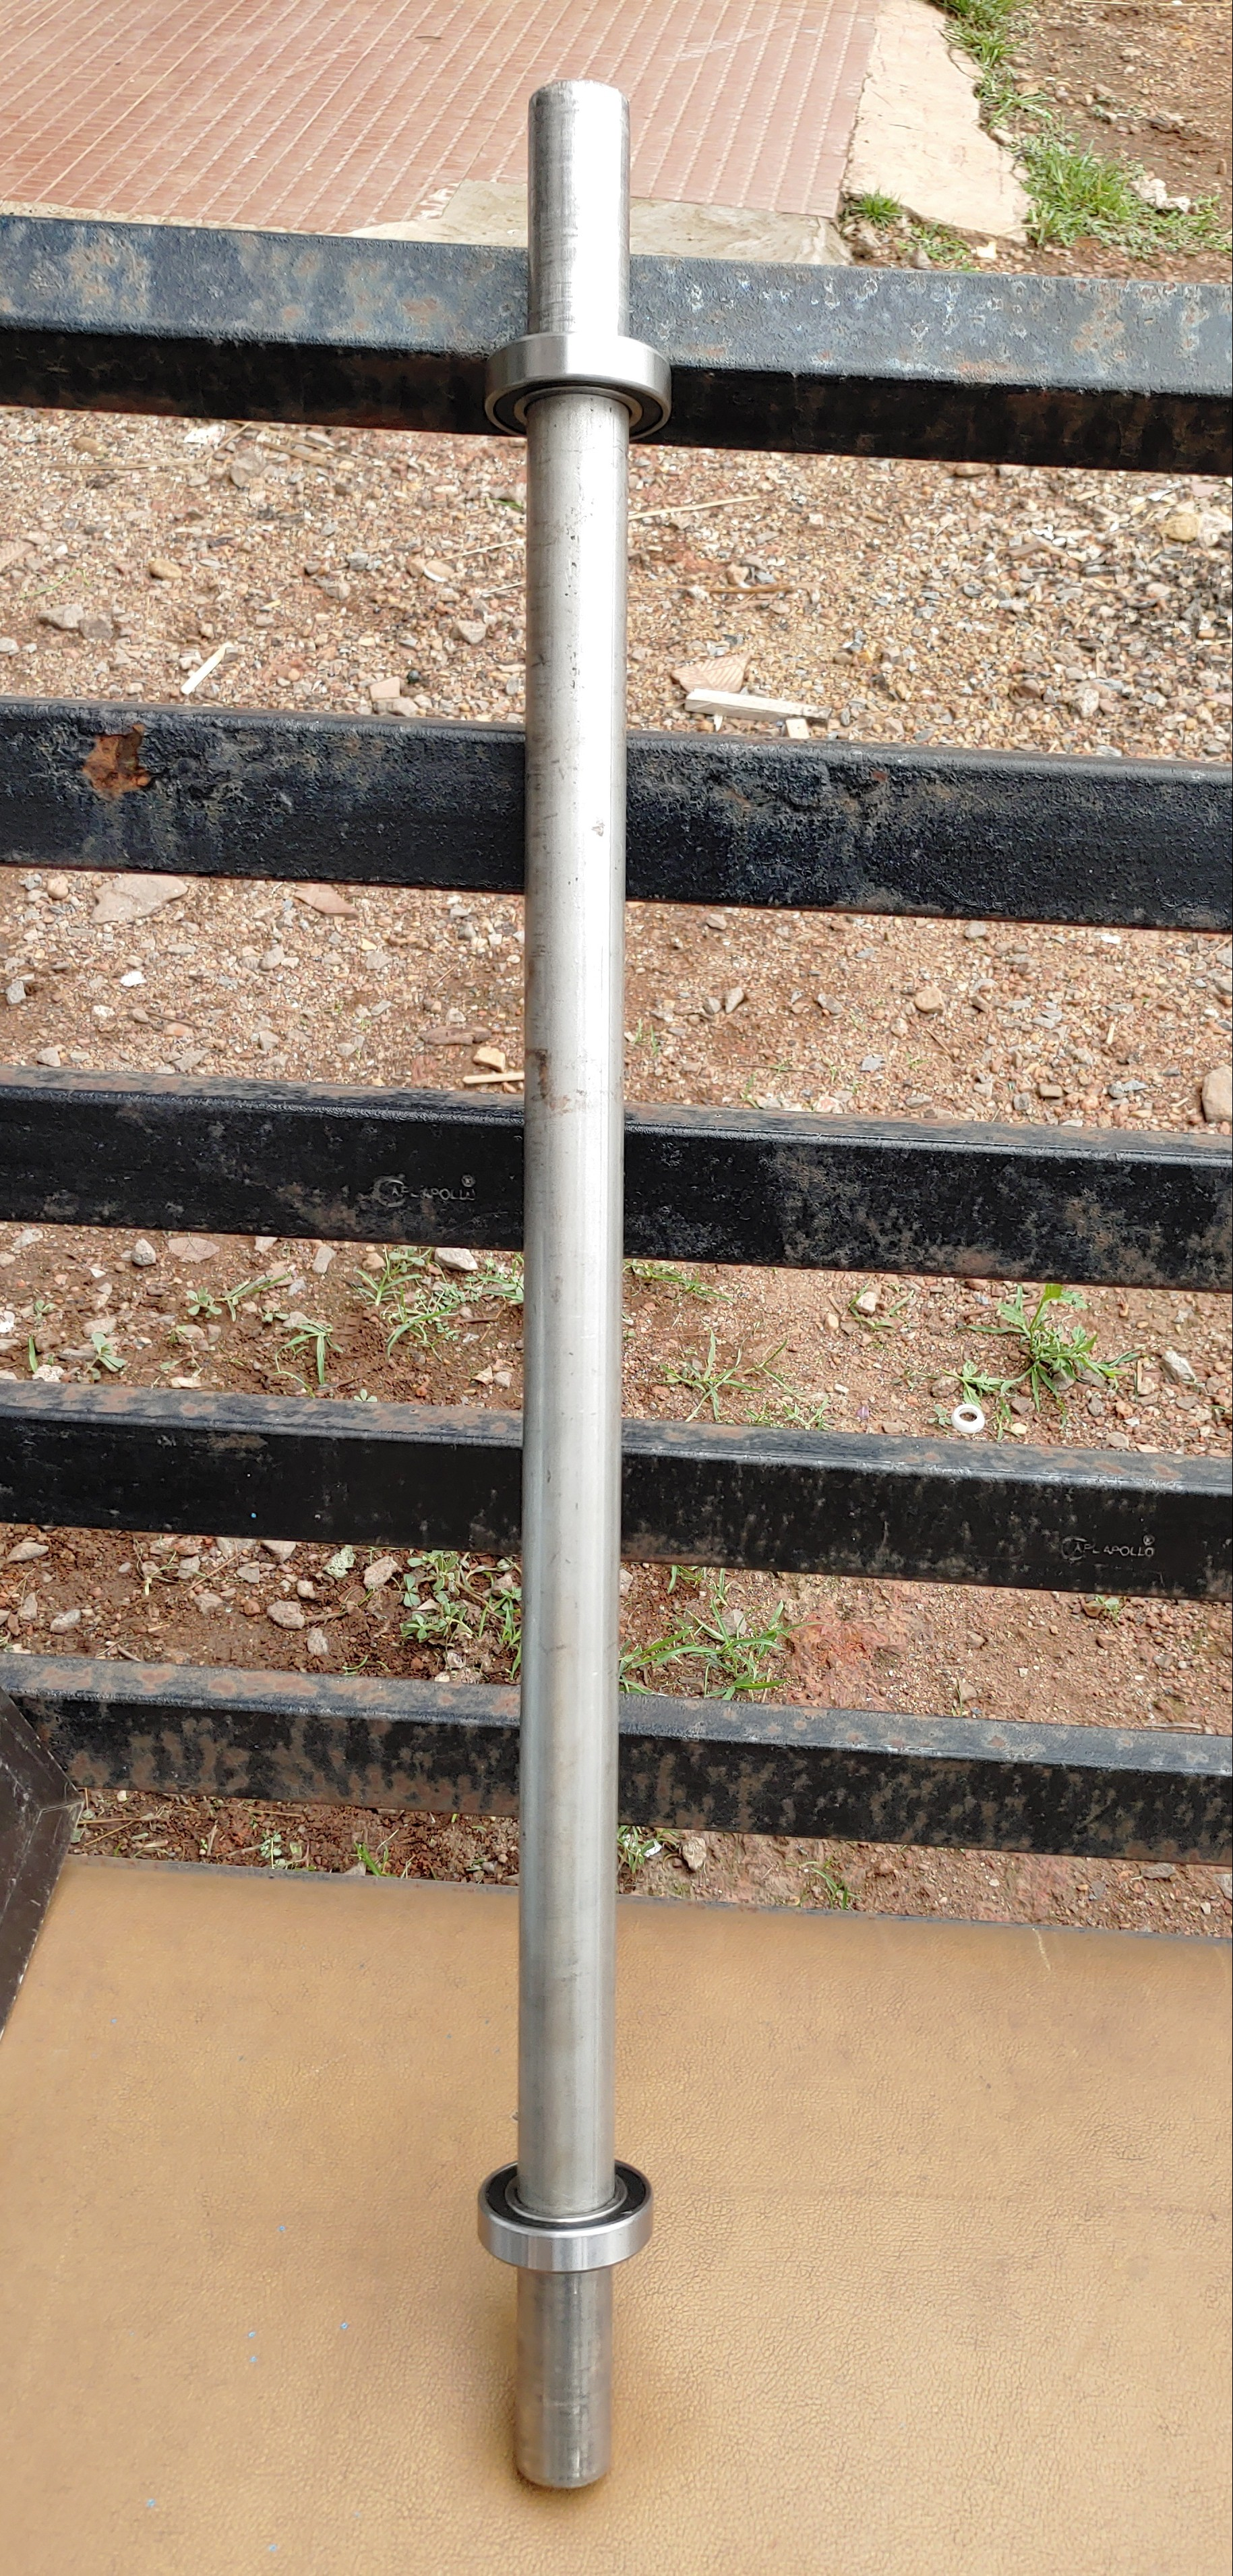
\includegraphics[width=0.8\textwidth]{bea shaf.jpg}
       \caption{Bearings on main shaft}
    \label{fig:Bearings on main shaft}
    \end{minipage}
\hfill
    \begin{minipage}{0.39\textwidth}
    \centering
      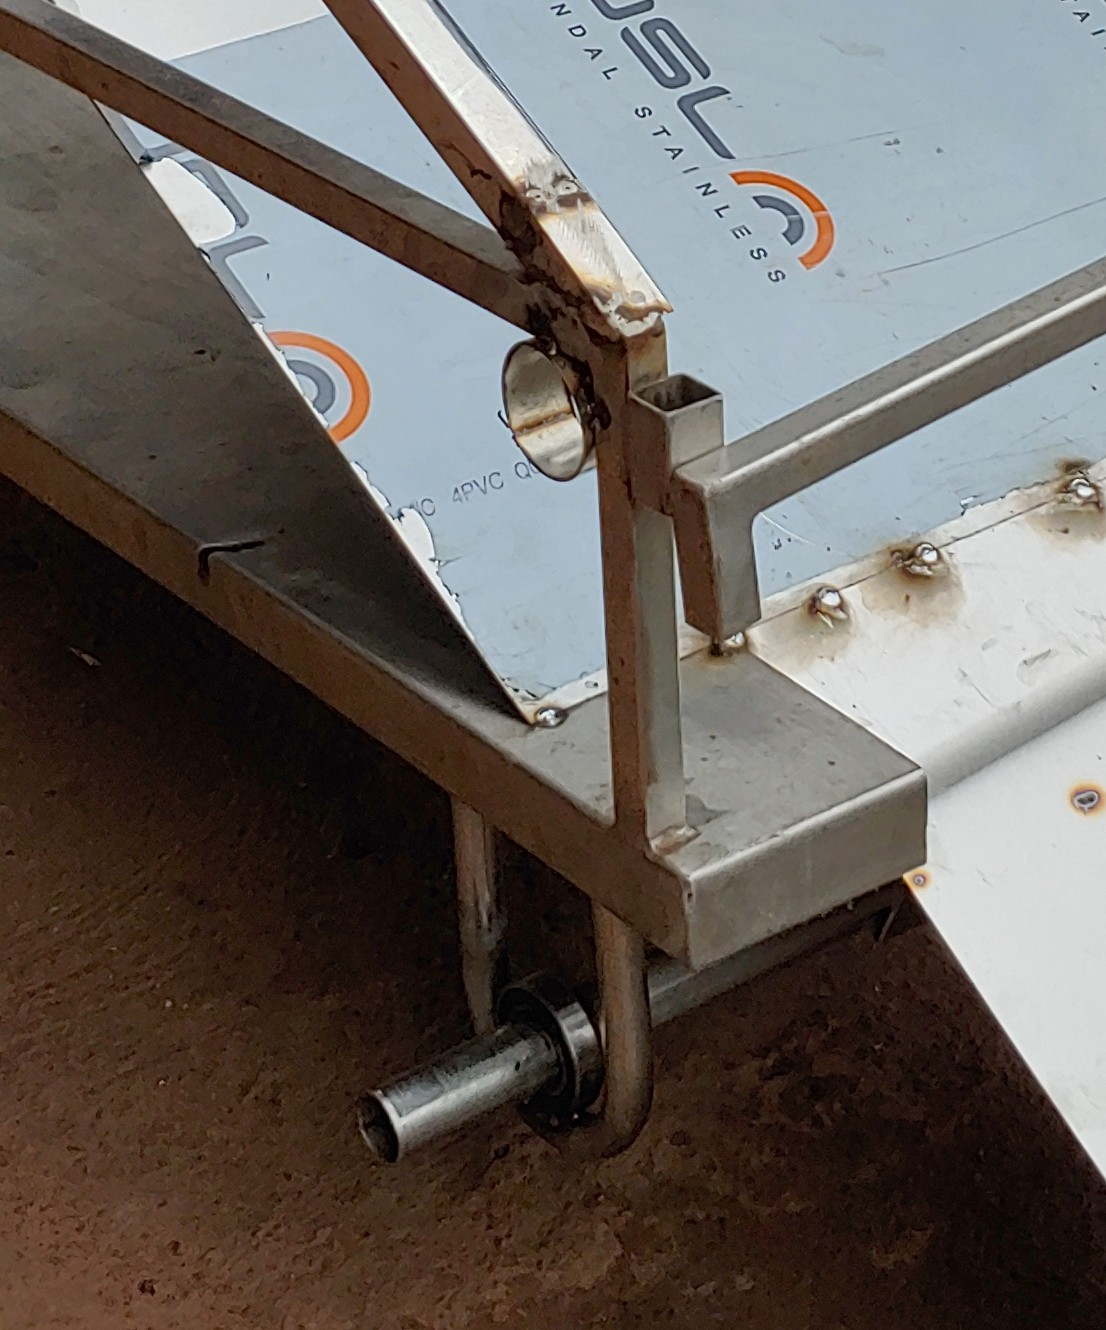
\includegraphics[width=0.8\textwidth]{mounts.jpg}
      \caption{Mounts}
      \label{fig:Mounts}
    \end{minipage}
\hfill
     \begin{minipage}{0.36\textwidth}
    \centering
      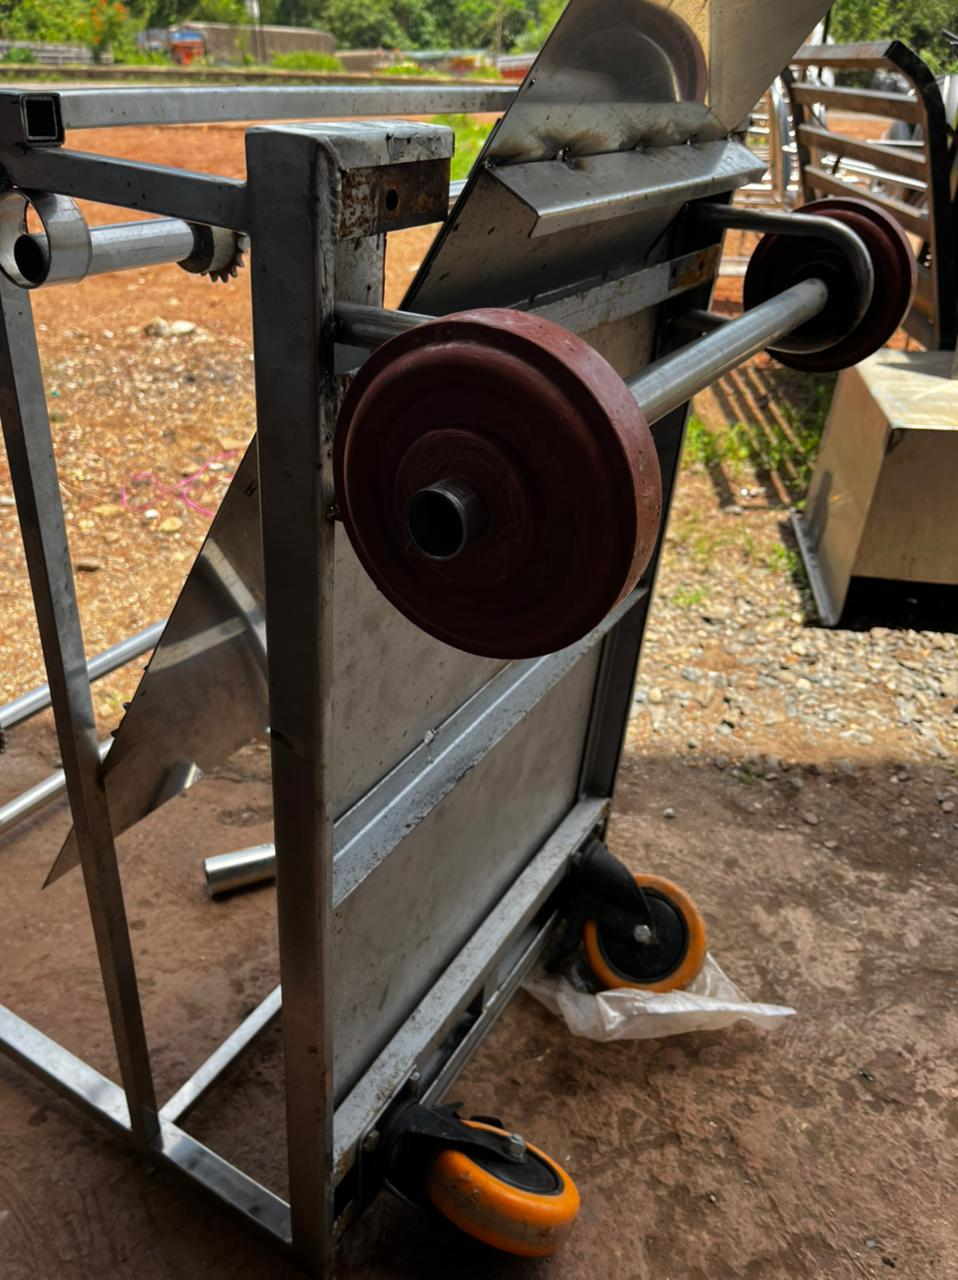
\includegraphics[width=0.8\textwidth]{tyres ass.jpg}
      \caption{Tyres assembly}
      \label{fig:Tyres assembly}
    \end{minipage}
\end{figure}





Two bearings and two sprockets were mounted on the shaft  (Fig. \ref{fig:Bearings and sprockets on auxiliary shaft}) and this arrangement was welded inside the circular mounts on the frame with a weld contact between the bearings and the mounts (Fig. \ref{fig:Auxiliary shaft assembly}).

\begin{figure}[H]
  \centering
    \begin{minipage}{0.185\textwidth}
    \centering
      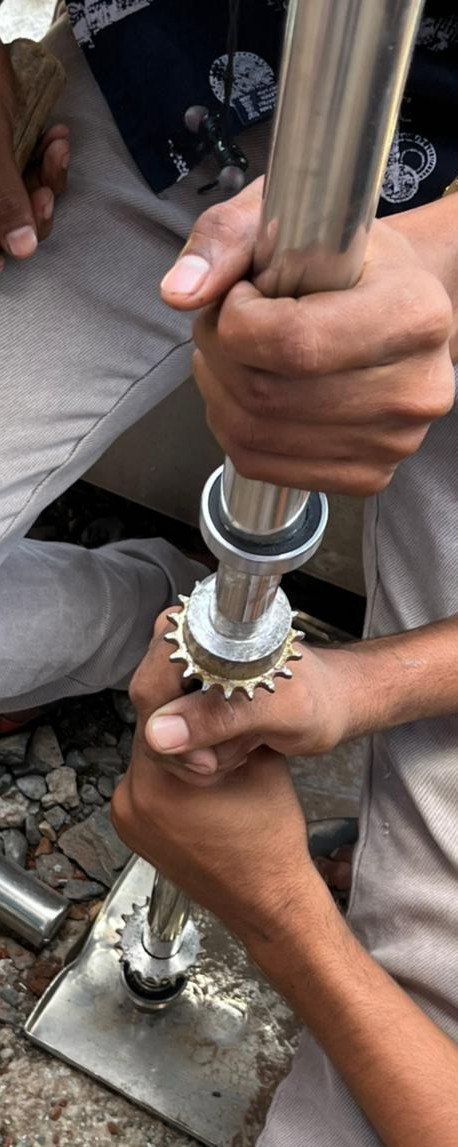
\includegraphics[width=1\textwidth]{bea spro sha.jpg}
       \caption{Bearings and sprockets on auxiliary shaft}
    \label{fig:Bearings and sprockets on auxiliary shaft}
    \end{minipage}
\hfill
    \begin{minipage}{0.40\textwidth}
    \centering
      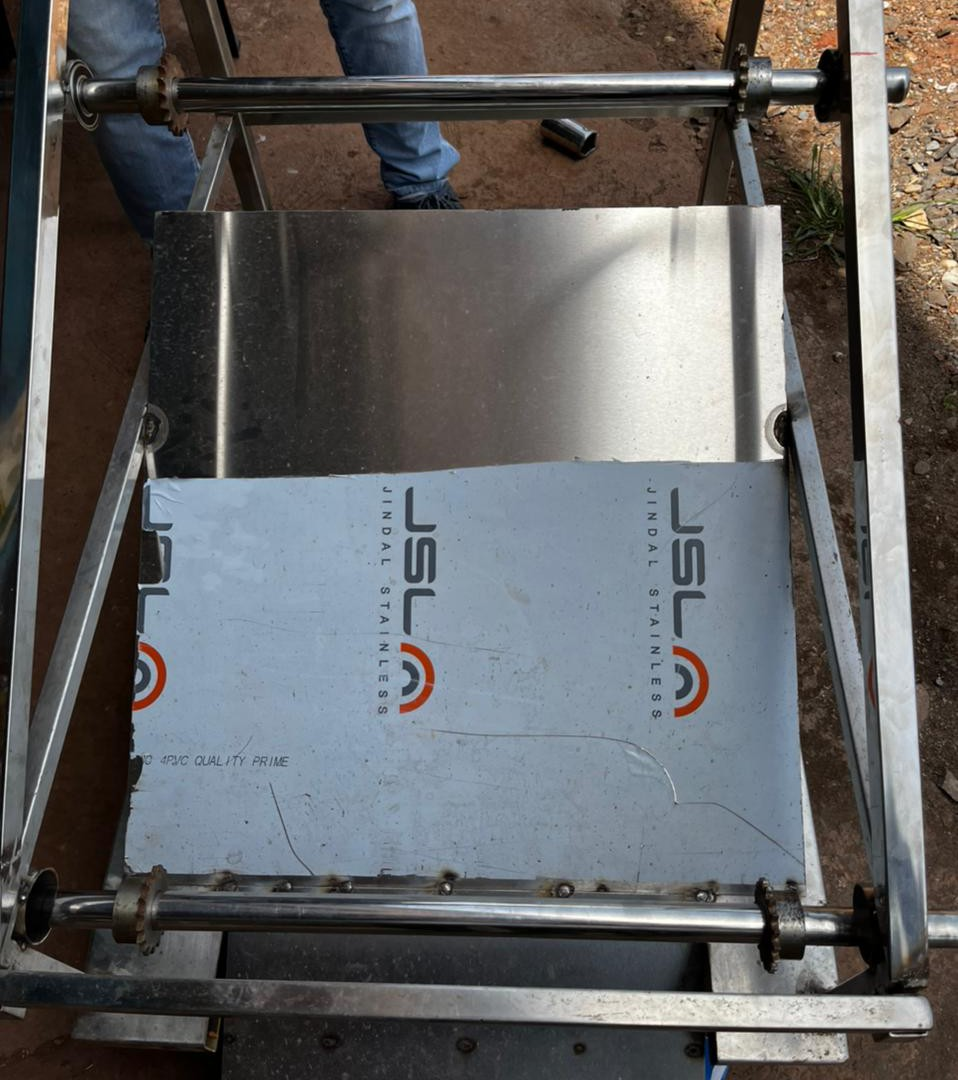
\includegraphics[width=1\textwidth]{bea spro ass.jpg}
      \caption{Auxiliary shaft assembly}
      \label{fig:Auxiliary shaft assembly}
    \end{minipage}
\end{figure}

Chains were mounted on the sprockets of the roller shafts (Fig. \ref{Chains mounted}).

Blades for the collecting mechanism were made by cutting SS sheet as per the required dimensions (Fig. \ref{blades}). Small cuts were made on the blade and the metal piece was bent for achieving better welding contact. 

\begin{figure}[H]
  \centering
    \begin{minipage}{0.30\textwidth}
    \centering
      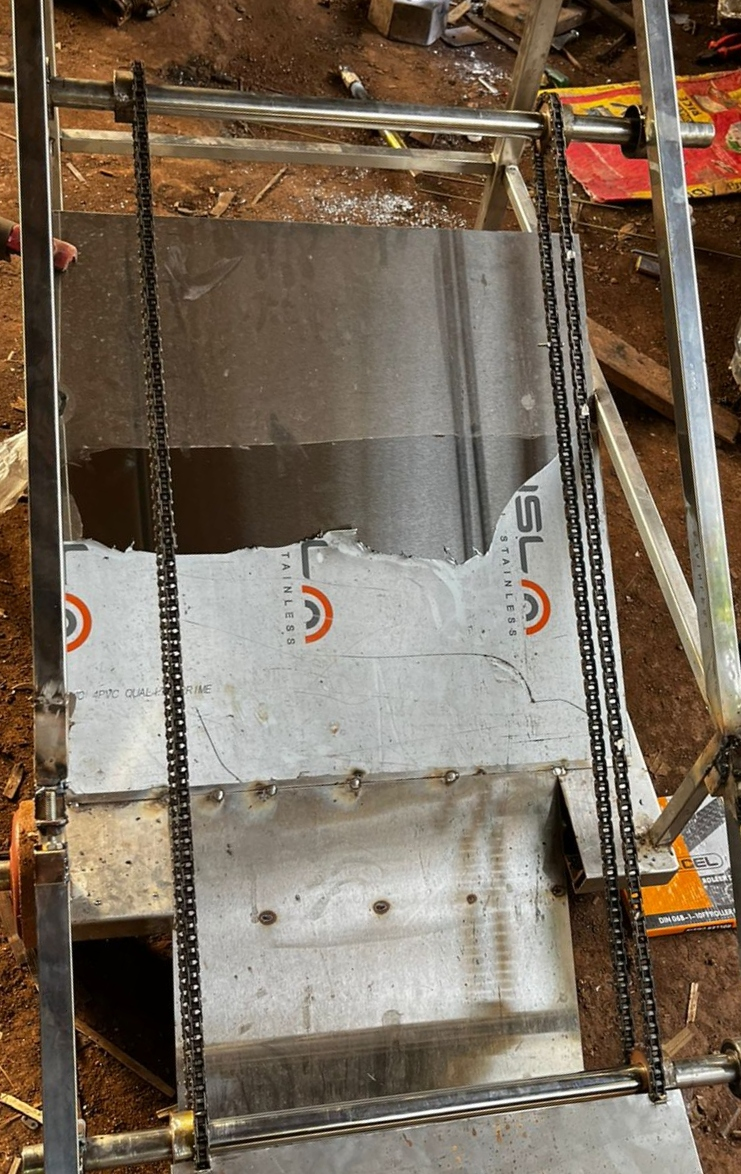
\includegraphics[width=1\textwidth]{chain frame ass.jpg}
       \caption{Chains mounted}
    \label{Chains mounted}
    \end{minipage}
\hfill
    \begin{minipage}{0.35\textwidth}
    \centering
      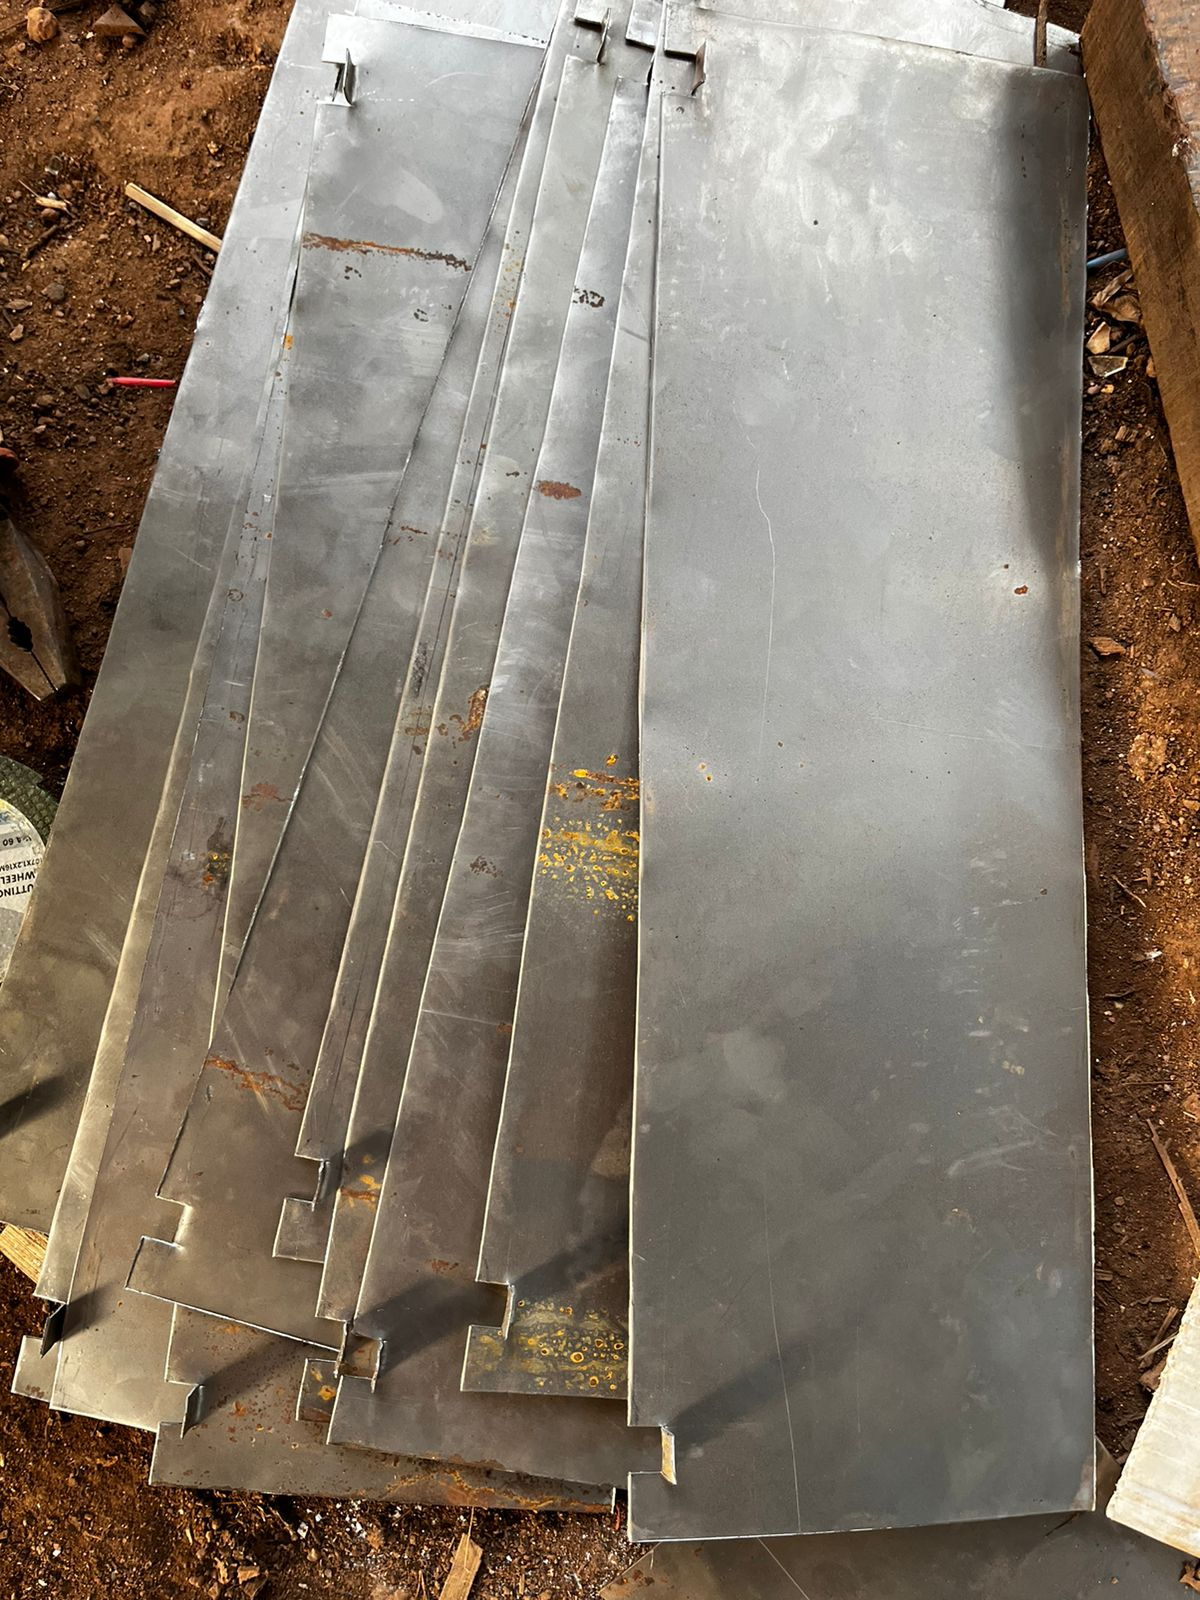
\includegraphics[width=1\textwidth]{blades.jpg}
      \caption{Blades}
      \label{blades}
    \end{minipage}
\end{figure} 

\noindent Blades were welded to the chains with an equal distance between the two successive blades (Fig. \ref{Blades ass}).

\begin{figure}[H]
  \centering
    \begin{minipage}{0.36\textwidth}
    \centering
      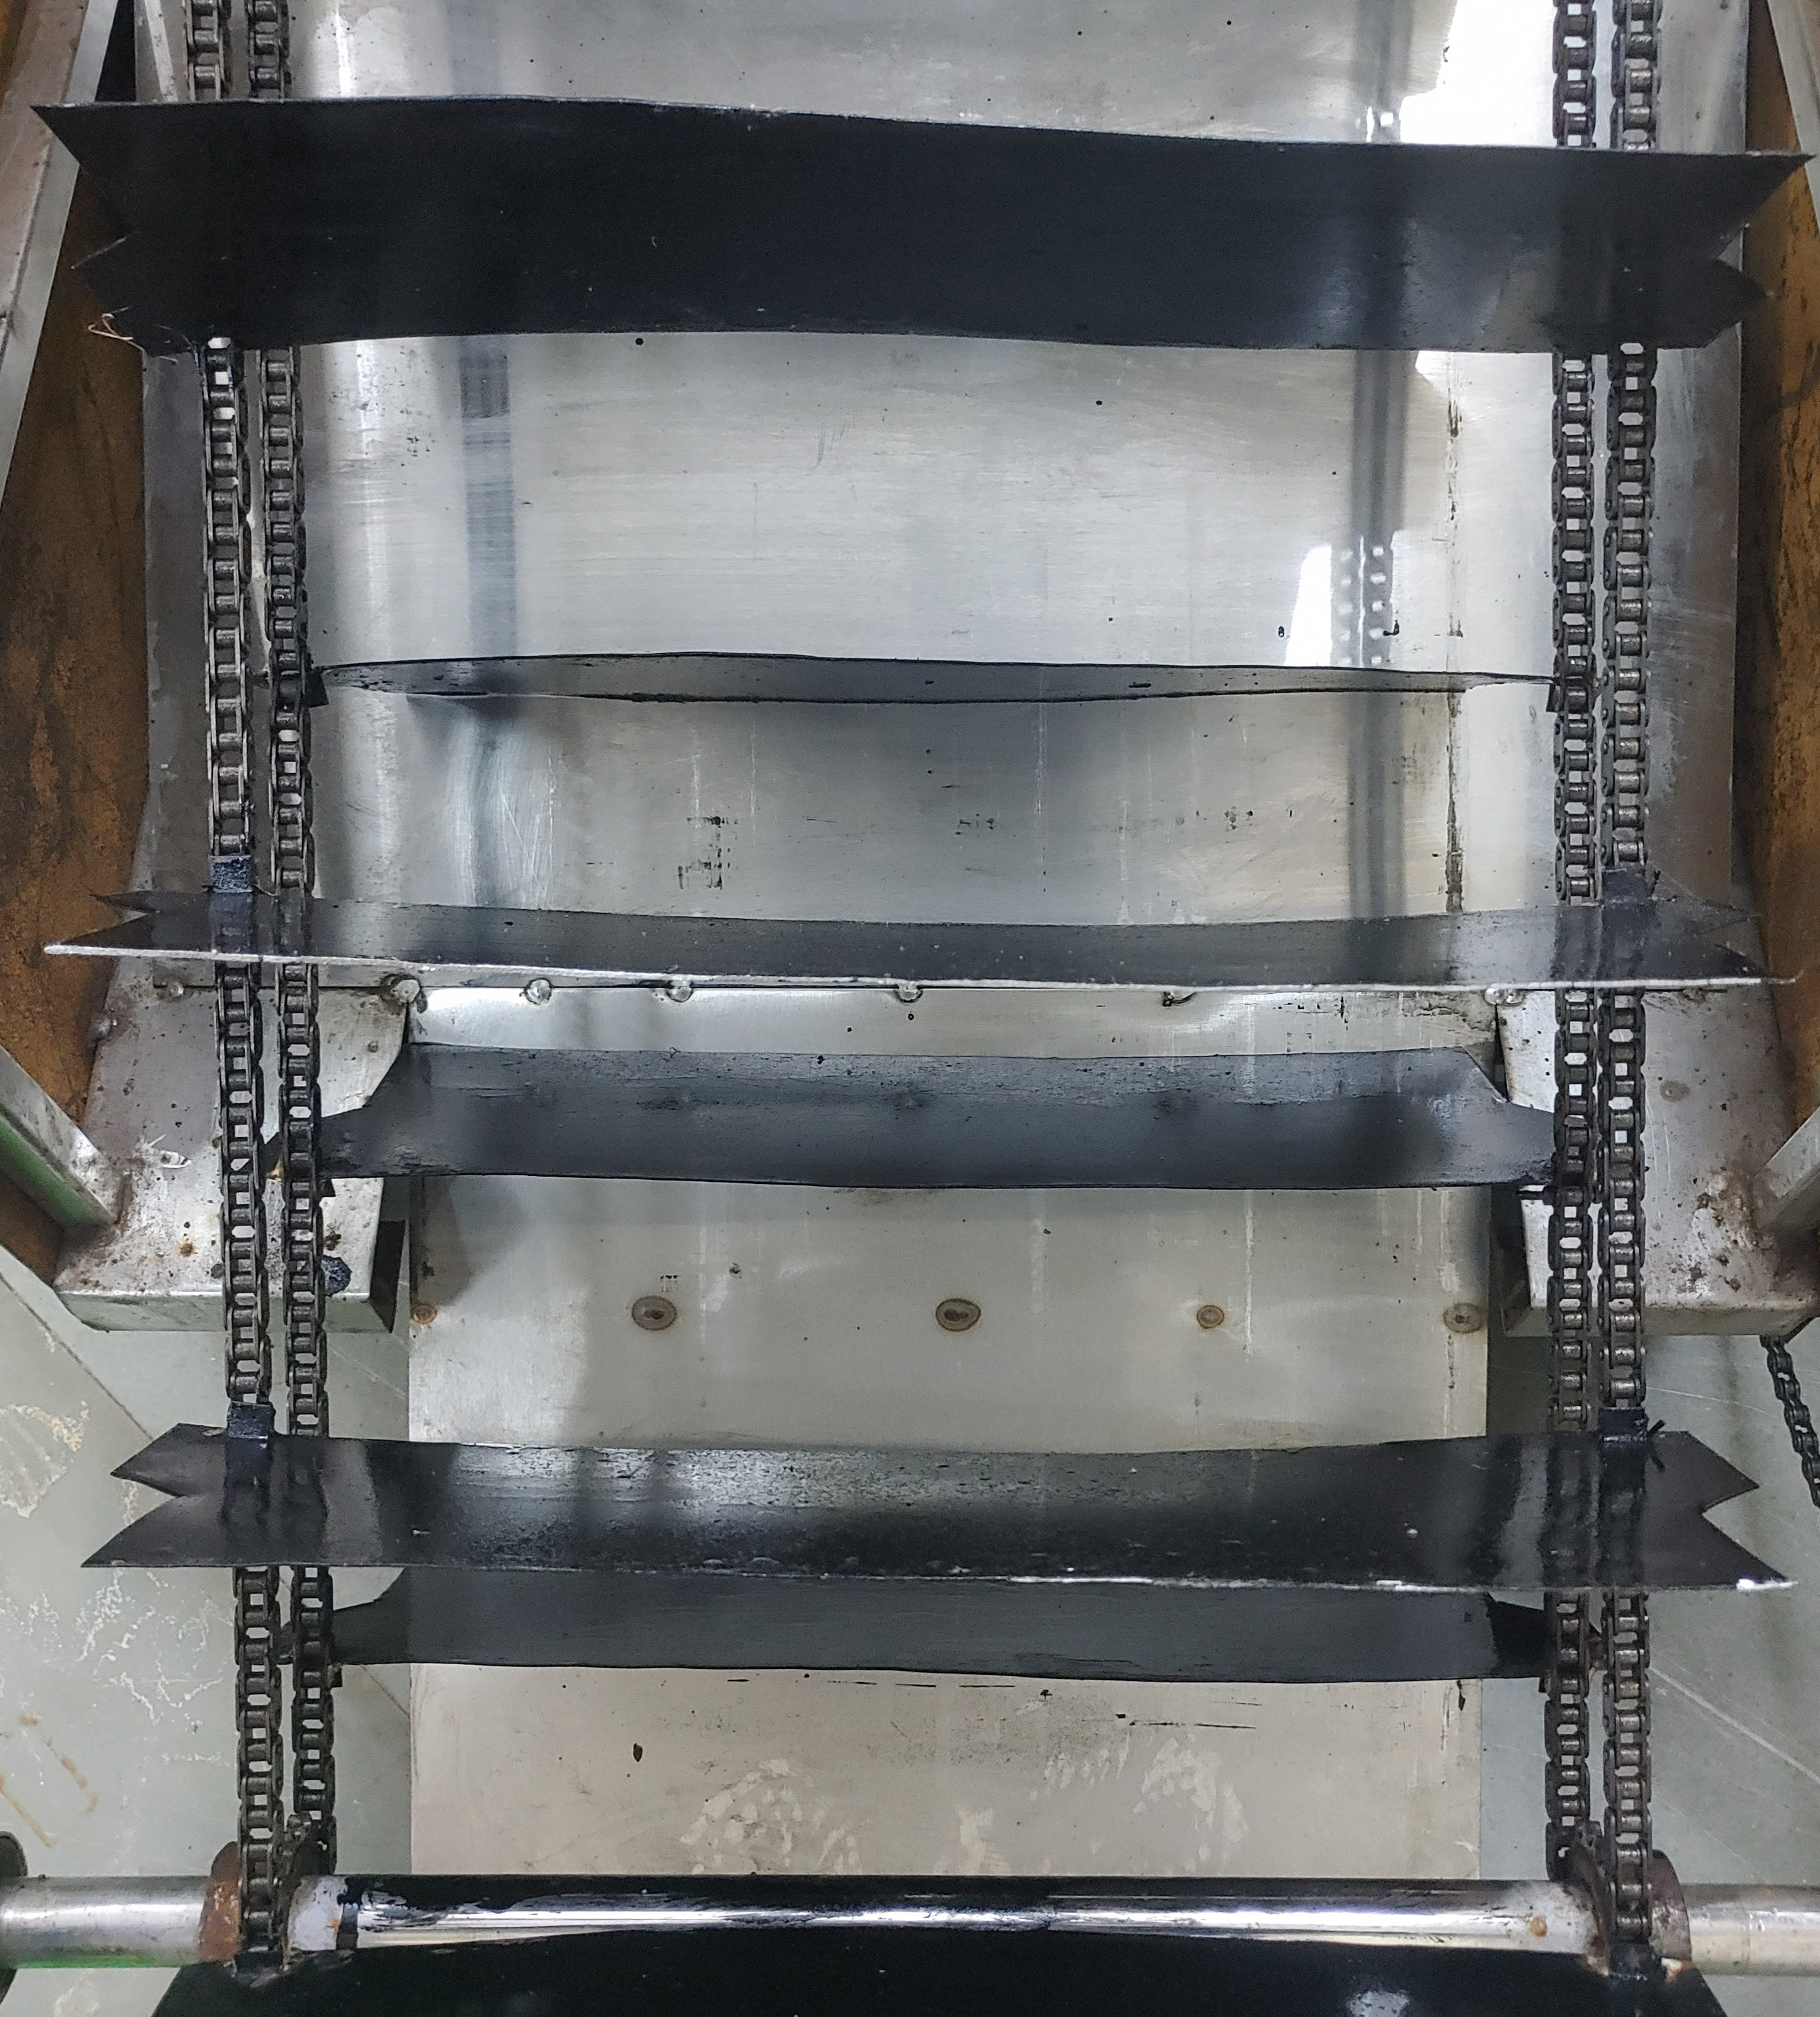
\includegraphics[width=1\textwidth]{Blades ass 2.jpg}
       \caption{Blade assembly}
    \label{Blade ass}
    \end{minipage}
\hfill
    \begin{minipage}{0.40\textwidth}
    \centering
      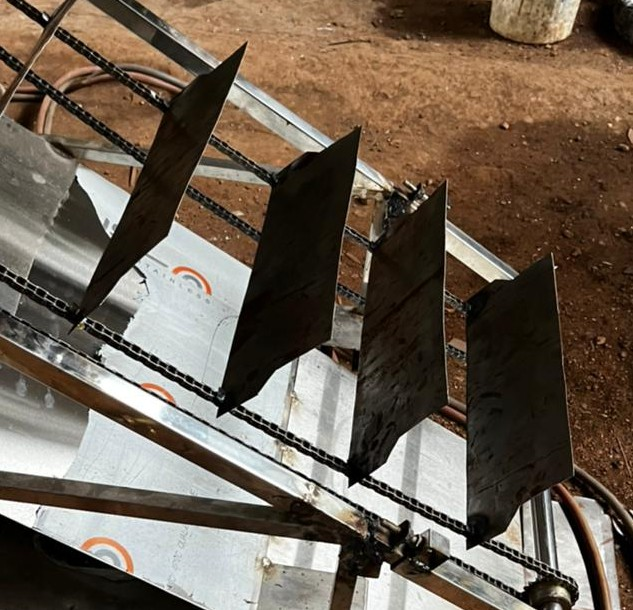
\includegraphics[width=1\textwidth]{Blades ass.jpg}
      \caption{Blade assembly}
      \label{Blades ass}
    \end{minipage}
\end{figure} 

A freewheel was mounted on the front roller shaft and a sprocket was mounted on the main shaft after the tyre. A chain was attached between the freewheel and the sprocket. This assembly drives the collecting mechanism (Fig. \ref{driving mechanism}).

\begin{figure}[H]
    \centering
    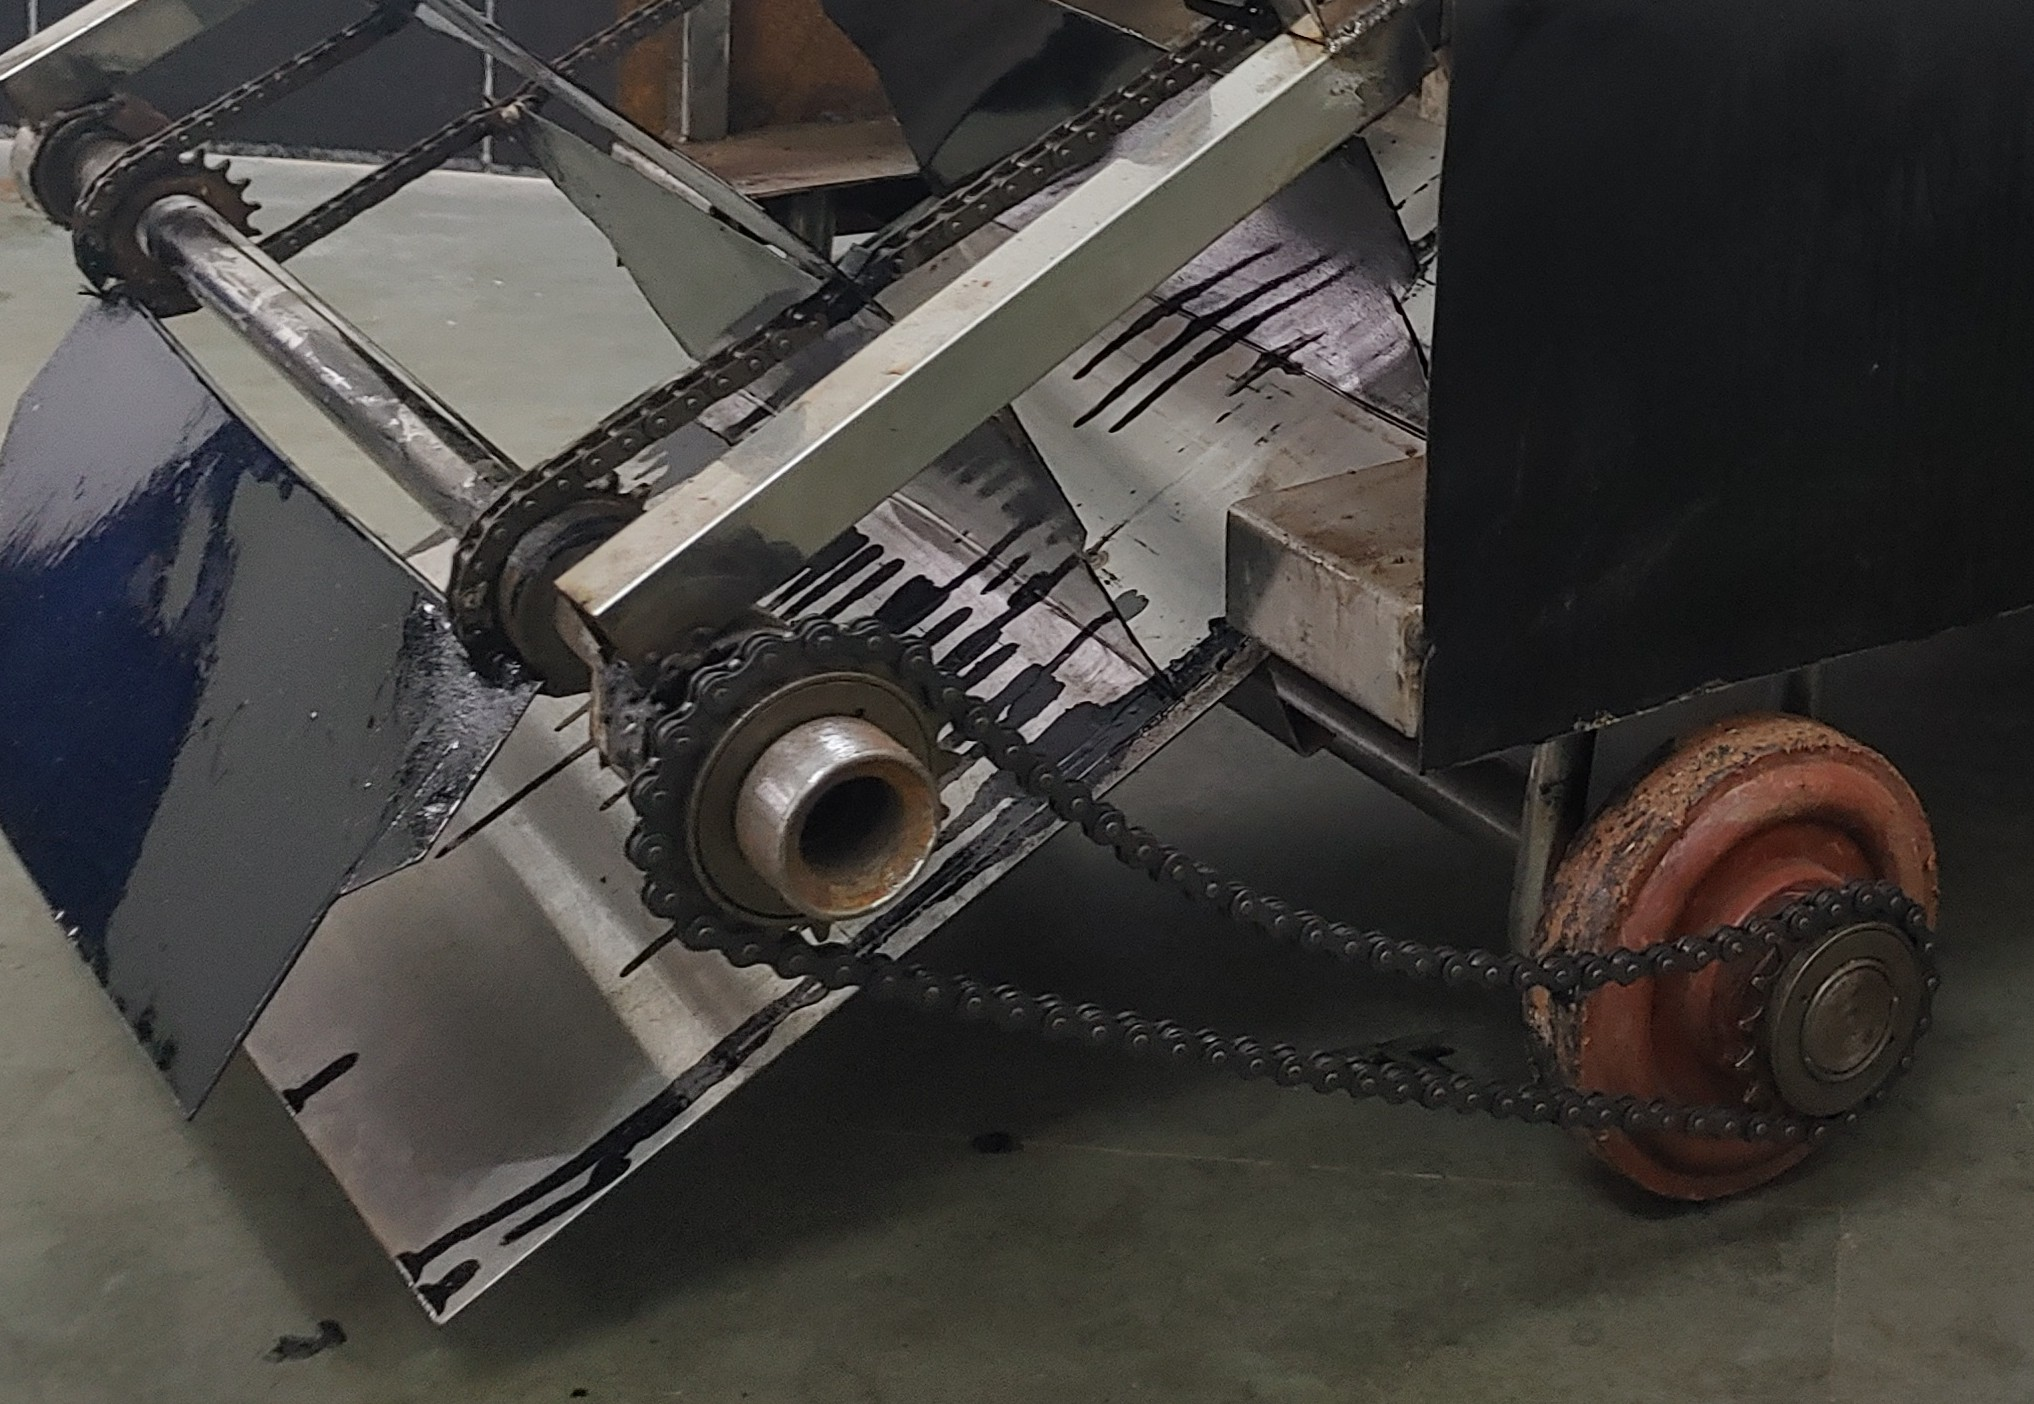
\includegraphics[scale=0.19]{driving mechanism.jpg}
    \caption{Driving mechanism}
    \label{driving mechanism}
\end{figure}





 


